%%%%%%%%%%%%%%%%%%%%%%%%%%%%%%%%%%%%%%%%%
% Masters/Doctoral Thesis
% LaTeX Template
% Version 1.43 (17/5/14)
%
% This template has been downloaded from:
% http://www.LaTeXTemplates.com
%
% Original authors:
% Steven Gunn
% http://users.ecs.soton.ac.uk/srg/softwaretools/document/templates/
% and
% Sunil Patel
% http://www.sunilpatel.co.uk/thesis-template/
%
% License:
% CC BY-NC-SA 3.0 (http://creativecommons.org/licenses/by-nc-sa/3.0/)
%
% Note:
% Make sure to edit document variables in the Thesis.cls file
%
%%%%%%%%%%%%%%%%%%%%%%%%%%%%%%%%%%%%%%%%%

%----------------------------------------------------------------------------------------
%	PACKAGES AND OTHER DOCUMENT CONFIGURATIONS
%----------------------------------------------------------------------------------------

\documentclass[11pt, oneside]{Thesis} % The default font size and one-sided printing (no margin offsets)

\graphicspath{{Images/}{Charts/}} % Specifies the directory where pictures are stored
\usepackage{times}
\usepackage{pdfpages}
\usepackage{subcaption}
\usepackage[square, numbers, comma, sort&compress]{natbib} % Use the natbib reference package - read up on this to edit the reference style; if you want text (e.g. Smith et al., 2012) for the in-text references (instead of numbers), remove 'numbers'
\usepackage{amsmath}
\usepackage{amssymb}
\usepackage{graphicx}
\usepackage{listings}
\usepackage{siunitx}
\usepackage{float}
\usepackage[euler]{textgreek}
% For algorithms management
\usepackage[linesnumbered, ruled]{algorithm2e}
\SetKwRepeat{Do}{do}{while}%

\lstset{
	language=Python,
	basicstyle=\ttfamily,
	keywordstyle=\color{blue}\ttfamily,
	stringstyle=\color{red}\ttfamily,
	commentstyle=\color{teal}\ttfamily,
	columns=flexible,
	}

\hypersetup{urlcolor=blue, colorlinks=true} % Colors hyperlinks in blue - change to black if annoying

\newcommand\YAMLcolonstyle{\color{red}\mdseries}
\newcommand\YAMLkeystyle{\color{black}\bfseries}
\newcommand\YAMLvaluestyle{\color{blue}\mdseries}

\makeatletter

% here is a macro expanding to the name of the language
% (handy if you decide to change it further down the road)
\newcommand\language@yaml{yaml}

\expandafter\expandafter\expandafter\lstdefinelanguage
\expandafter{\language@yaml}
{
  keywords={true,false,null,y,n},
  keywordstyle=\color{darkgray}\bfseries,
  basicstyle=\YAMLkeystyle,                                 % assuming a key comes first
  sensitive=false,
  comment=[l]{\#},
  morecomment=[s]{/*}{*/},
  commentstyle=\color{purple}\ttfamily,
  stringstyle=\YAMLvaluestyle\ttfamily,
  moredelim=[l][\color{orange}]{\&},
  moredelim=[l][\color{magenta}]{*},
  moredelim=**[il][\YAMLcolonstyle{:}\YAMLvaluestyle]{:},   % switch to value style at :
  morestring=[b]',
  morestring=[b]",
  literate =    {---}{{\ProcessThreeDashes}}3
                {>}{{\textcolor{red}\textgreater}}1
                {|}{{\textcolor{red}\textbar}}1
                {\ -\ }{{\mdseries\ -\ }}3,
}

% switch to key style at EOL
\lst@AddToHook{EveryLine}{\ifx\lst@language\language@yaml\YAMLkeystyle\fi}
\makeatother

\newcommand\ProcessThreeDashes{\llap{\color{cyan}\mdseries-{-}-}}

\title{\ttitle} % Defines the thesis title - don't touch this

\begin{document}
\frontmatter % Use roman page numbering style (i, ii, iii, iv...) for the pre-content pages

\setstretch{1.3} % Line spacing of 1.3

% Define the page headers using the FancyHdr package and set up for one-sided printing
\fancyhead{} % Clears all page headers and footers
\rhead{\thepage} % Sets the right side header to show the page number
\lhead{} % Clears the left side page header

\pagestyle{fancy} % Finally, use the "fancy" page style to implement the FancyHdr headers

\newcommand{\HRule}{\rule{\linewidth}{0.5mm}} % New command to make the lines in the title page
\newcommand{\datasetunimore} {Interactive Museum}
\newcommand{\argmax}{\arg\!\max}
% PDF meta-data
\hypersetup{pdftitle={\ttitle}}
\hypersetup{pdfsubject=\subjectname}
\hypersetup{pdfauthor=\authornames}
\hypersetup{pdfkeywords=\keywordnames}

%----------------------------------------------------------------------------------------
%	TITLE PAGE
%----------------------------------------------------------------------------------------

\begin{titlepage}

\begin{center}
\textsc{\Large \bf \univname}\\[0.5cm] % University name
\textsc{\large Dipartimento di Ingegneria ``Enzo Ferrari"}\\[0.2cm] % Thesis type
%\HRule \\ % Horizontal line
\textsc{\large Corso di Laurea Magistrale in Ingegneria Informatica}\\[5.0cm] % Thesis type

\HRule \\[0.6cm] % Horizontal line
{\huge \bfseries \ttitle}\\[0.4cm] % Thesis title
%\HRule \\[0.6cm] % Horizontal line
%{\huge \bfseries \ttitleITA}\\[0.4cm] % Thesis title
\HRule \\[3.2 cm] % Horizontal line

\begin{minipage}{0.4\textwidth}
\begin{flushleft} \large
\emph{Candidato:}\\
\authornames % Author name - remove the \href bracket to remove the link
\end{flushleft}
\end{minipage}
\begin{minipage}{0.4\textwidth}
\begin{flushright} \large
\emph{Relatore:} \\
\supname \\ % Supervisor name - remove the \href bracket to remove the link
\emph{Correlatore:} \\
\cosupname \\ % Supervisor name - remove the \href bracket to remove the link
\end{flushright}
\end{minipage}\\[5.0cm]

%\large \textit{A thesis submitted in fulfilment of the requirements\\ for the degree of \degreename}\\[0.3cm] % University requirement text
%\textit{in the}\\[0.4cm]
%\groupname\\\deptname\\[2cm] % Research group name and department name

\textsc{\large Anno Accademico 2021-2022}\\[4cm] % Date
%\includegraphics{Logo} % University/department logo - uncomment to place it

\vfill
\end{center}

\end{titlepage}

\clearpage % Start a new page

%----------------------------------------------------------------------------------------
%	SYMBOLS
%----------------------------------------------------------------------------------------

%\clearpage % Start a new page
%
%\lhead{\emph{Symbols}} % Set the left side page header to "Symbols"
%
%\listofnomenclature{lll} % Include a list of Symbols (a three column table)
%{
%$a$ & distance & m \\
%$P$ & power & W (Js$^{-1}$) \\
%% Symbol & Name & Unit \\
%
%& & \\ % Gap to separate the Roman symbols from the Greek
%
%$\omega$ & angular frequency & rads$^{-1}$ \\
%% Symbol & Name & Unit \\
%}
\newcommand{\etal}{\textit{et al.~}}

%----------------------------------------------------------------------------------------
%	ABSTRACT PAGES
%----------------------------------------------------------------------------------------
\addtotoc{Abstract in English} % Add the "Abstract" page entry to the Contents
\englishAbstract{\addtocontents{toc}{\vspace{1em}} % Add a gap in the Contents, for aesthetics
Dental implant placement within the jawbone is a routinely executed surgical
procedure, which can become complex due to the local presence of the Inferior
Alveolar Nerve (IAN). In particular, the nerve is oftentimes in close relation
to the roots of molars, and its position must thus be carefully detailed before
the surgical removal. As avoiding contact with the IAN is a primary concern
during these operations, segmentation plays a key role in surgical
preparations.\\ Unfortunately, 3D manual segmentation requires a huge amount of
time to be carried out, thus perfect anatomical annotations are usually
overlooked in favor of fast executions. The de facto standard in radiology
medical centers for dentistry and maxilla facial purposes is based on sparse
annotations, which can be obtained from 2D images in a relatively small amount
of time. This type of annotation fails to identify a considerable amount of
inner information about the IAN position and the bone structure.
Convolutional Neural Networks are known to provide amazing results in the
segmentation task and could provide to medical operators an automatic and
precise way to detect the IAN in patients, allow them to be more accurate during
the operations where this information is critical. This type of network requires
a large amount of labeled data to reach a good level of accuracy while in the
medical field is hard and expensive to acquire, meanwhile a good amount of
unlabeled data is available.\\
In this work we study and analyze the effectiveness of some of the most recent
proposal made in the literature for segmentation in the medical imaging field,
some of which have recently obtained state-of-the-art results for other similar
tasks. Even if we do not reach the same level of accuracy we expected, we show
that we were able to improve the speed of the training process and the
performance of the network, while keeping the same level of accuracy of the
original network.

%Depositate anche su esse3, quindi se le cambi cambia anche lì
\textbf{Keywords:} Medical Imaging, Deep Learning, 3D Segmentation, Computer
Vision, Cone Beam Computed Tomography.
}
\clearpage % Start a new page

\addtotoc{Abstract in Italian} % Add the "Abstract" page entry to the Contents
\italianAbstract{\addtocontents{toc}{\vspace{1em}} % Add a gap in the Contents, for aesthetics
L'inserimento di impianti dentali nella mascella è una ruotine chirurgica
abbastanza comune, ma è resa non banale dalla presenza del nervo alveolare
inferiore. Questo nervo è posizionato in prossimità delle radici dei molari,
e la sua posizione deve essere accuratamente delineata prima di poter eseguire
l'operazione voluta, in quanto danneggiare tale nervo potrebbe essere causa di
gravi conseguenze per il paziente, come ad esempio la perdita della
sensibilità o la paralisi di tale zona. Poichè evitare il contatto con questo
nervo è essenziale, un'accurata segmentazione di tale nervo è un requisito
chiave. Sfortunatamente, una segmentazione 3D manuale richiede un'enorme
quantità di tempo, per questo motivo solitamente si preferiscono metodi meno
precisi ma più veloci e per questo motivo lo standard de-facto per i dentisti è
basato sull'effettuare una annotazione sparsa, ottenuta da immagini 2D. Questo
tipo di annotazione fallisce nell'identificare una buona parte delle
informazioni che riguardano la posizione del nervo e la struttura ossea del
canale in cui esso è contenuto.\\
Le reti neurali convolutive hanno dimostrato di poter ottenere risultati ottimi
nell'effettuare la segmentazione di immagini e in questo caso potrebbe offrire
ai medici un metodo automatico, preciso e veloce di delineare il nervo alveolare
inferiore, essenziale soprattutto durante le operazioni più critiche. Questo
tipo di reti neurali richiede una quantità enorme di dati annotati per poter
imparare a svolgere correttamente questo tipo di task con una accuratezza
soddisfacente. In ambito medico, è possibile ottenere una decente quantità di
immagini, ma non di annotazioni. Per questo motivo è necessario progettare
accuratamente i metodi utilizzati durante il design e l'allenamento di tali reti
in modo da superare questa mancanza senza perdere in prestazioni.
In questa
tesi, diverse tecniche molto recenti vengono provate ed analizzate, per
studiarne l'efficacia in questo specifico lavoro. Alcuni metodi che recentemente
hanno avuto molto successo nell'ambito della computer vision, non hanno avuto
gli stessi risultati sperati in questo specifico caso, mentre altri approcci si
sono rivelati molto efficaci nell'ottimizzare e velocizzare il processo di
training della rete, senza perdere accuratezza nella segmentazione.

\textbf{Parole Chiave:} Medical Imaging, Deep Learning, 3D Segmentation,
Computer Vision, Cone Beam Computed Tomography.
}
\clearpage % Start a new page

%----------------------------------------------------------------------------------------
%	SINTESI IN ITALIANO PAGES
%----------------------------------------------------------------------------------------

\addtotoc{Summary in Italian} % Add the "Abstract" page entry to the Contents
%
\italianSummary{\addtocontents{toc}{\vspace{1em}} % Add a gap in the Contents, for aesthetics
%
Il regolamento della Facoltà di Ingegneria di Modena prevede che le tesi scritte
in lingua inglese debbano contenere un \textit{abstract} ed un'ampia sintesi dei
contenuti in lingua italiana: in accordo a questa regola, proponiamo un sunto
degli argomenti, delle tecniche e dei risultati che verranno delineati
nell'elaborato. Si noti che non si tratta di un sunto esaustivo, e che non è
possibile valutare la tesi dalla semplice lettura di queste righe. Per una
descrizione più dettagliata e più rigorosa, e per i risultati sperimentali
ottenuti, si rimanda al testo in inglese.

Questa tesi tratta della segmentazione del canale alveolare inferiore su
immagini di tomografia conica a fascio di coni (Cone Beam Computed Tomography,
CBCT) tramite l'utilizzo di reti neurali. Tale procedura è essenziale per
l'inserimento di impianti dentali nella mascella, poichè il nervo alveolare
inferiore deve essere accuratamente delineato prima di poter eseguire
l'operazione voluta, in quanto danneggiare tale nervo potrebbe essere causa di
gravi conseguenze per il paziente, come ad esempio la perdita della sensibilità
o la paralisi di tale zona.\\
La segmentazione di immagini è un problema di grande interesse in ambito della
visione artificiale, in quanto permette di ottenere informazioni utili per
diversi scopi. In ambito medico, la segmentazione di immagini risulta uno
strumento molto utile a supporto dei medici. Per questo motivo c'è stata una
forte ricerca sulla segmentazione di immagini mediche (CT, CBCT, MRI, ecc.), che
ha seguito i trend della visione artificiale "classica". Ad oggi, quest'area è
dominata dalle reti neurali, che hanno dimostrato di poter ottenere risultati
molto migliori delle tecniche classiche. Negli ultimi anni, la tipologia di reti
neurali che ha avuto maggior successo è stata quella delle reti neurali
completamente convolutive (CNN), ovvero reti neurali che non hanno alcun layer
completamente connesso ma solo layer convoluzionali. Tra queste, si è visto che
le reti a forma di U, come U-Net, sono quelle che ottengono i migliori
risultati, dato dal fatto che sono in gradi di essere molto profonde senza
soffrire del problema del gradiente evanescente grazie alle connessioni
residuali. Queste reti seguono un approccio di codifica-decodifica, in cui
l'input viene codificato in una rappresentazione più compatta, che viene
successivamente decodificata in un output di dimensione equivalente a quella di
input.\\
Negli ultimi anni però i transformers, un tipo di rete neurale che sfrutta la
tecnica dell'attenzione proposto per la prima volta nel campo del linguaggio
naturale, hanno ottenuto risultati molto interessanti anche nell'ambito delle
immagini. Non sono stati fin da subito adottati anche nel campo medico perché
hanno la scomoda caratteristica di aver bisogno di molti dati per ottenere
risultati comparabili o superiori alle reti convolutive. I dataset di immagini
mediche sono pochi e ognuno contiene pochi esempi. Nel caso del canale alveolare
inferiore, solo un dataset, Maxillo, ad oggi è disponibile e contiene $91$
esempi con una etichettatura densa mentre $200$ con solo un'etichettatura sparsa
(mentre nei dataset non medici, solitamente ha un numero di esempio dell'ordine
di $10^5$). Questo problema è dato dal fatto che per annotare immagini mediche
è necessario che un medico esperto le analizzi e le etichetti a mano, cosa che
richiede molto tempo ed è anche molto costosa.
Un altra caratteristica delle immagini mediche è che la zona da etichettare è
solitamente molto piccola rispetto al volume completo, e questo rende più
difficile l'apprendimento della rete.\\
Il lavoro di questa tesi è stato inizialmente quello di fare un refactoring del
codice precedentemente scritto, in modo da ottimizzare alcuni processi, come la
lettura e il caricamento dei dati, migliorare l'usabilità e la mantenibilità e
poter effettuare i test necessari in modo molto più efficace.
Successivamente si è studiata l'efficacia di diverse tecniche proposte in
letteratura, con lo scopo di migliorare lo stato dell'arte. Durante la tesi, ho
potuto anche contribuire ad una libreria open source, TorchIO, estremamente
utilizzata per caricare e processare immagini mediche insieme alle reti neurali
profonde, aggiungendo una nuova funzionalità, inizialmente proposta da altri,
che si è dimostrata molto efficace anche nei nostri esperimenti.


}
%
\clearpage % Start a new page

%----------------------------------------------------------------------------------------
%	DEDICATION
%----------------------------------------------------------------------------------------
\mainmatter
\setstretch{1.3} % Return the line spacing back to 1.3

\pagestyle{empty} % Page style needs to be empty for this page

% \dedicatory{To ...} % Dedication text

% \addtocontents{toc}{\vspace{2em}} % Add a gap in the Contents, for aesthetics

%----------------------------------------------------------------------------------------
%	ACKNOWLEDGEMENTS
%----------------------------------------------------------------------------------------

\setstretch{1.3} % Reset the line-spacing to 1.3 for body text (if it has changed)

\acknowledgements{\addtocontents{toc}{\vspace{1em}} % Add a gap in the Contents, for aesthetics
First and foremost, I would like to express my gratitude to my supervisors,
Prof. Federico Bolelli and Prof. Costantino Grana, for their guidance, support,
and encouragement throughout my work. I would also like to thank them for
introducing me to the world of academic research by bringing me with them to a
conference, and for inspiring me to continue my studies by enrolling in a Ph.D.
program. Thanks goes also to my family and my friends  for their unwavering
support because, without them, I would not be the person I am today.
}
\clearpage % Start a new page

%----------------------------------------------------------------------------------------
%	LIST OF CONTENTS/FIGURES/TABLES PAGES
%----------------------------------------------------------------------------------------

\pagestyle{fancy} % The page style headers have been "empty" all this time, now use the "fancy" headers as defined before to bring them back

\lhead{\emph{Contents}} % Set the left side page header to "Contents"
\tableofcontents % Write out the Table of Contents

\lhead{\emph{List of Figures}} % Set the left side page header to "List of Figures"
\listoffigures % Write out the List of Figures

\lhead{\emph{List of Tables}} % Set the left side page header to "List of Tables"
\listoftables % Write out the List of Tables

\lhead{\emph{List of Listings}} % Set the left side page header to "List of Listings"
\lstlistoflistings % Write out the List of Listings

%----------------------------------------------------------------------------------------
%	ABBREVIATIONS
%----------------------------------------------------------------------------------------

%\clearpage % Start a new page
%
%\setstretch{1.5} % Set the line spacing to 1.5, this makes the following tables easier to read
%
%\lhead{\emph{Abbreviations}} % Set the left side page header to "Abbreviations"
%\listofsymbols{ll} % Include a list of Abbreviations (a table of two columns)
%{
%\textbf{LAH} & \textbf{L}ist \textbf{A}bbreviations \textbf{H}ere \\
%%\textbf{Acronym} & \textbf{W}hat (it) \textbf{S}tands \textbf{F}or \\
%}

%----------------------------------------------------------------------------------------
%	PHYSICAL CONSTANTS/OTHER DEFINITIONS
%----------------------------------------------------------------------------------------

%\clearpage % Start a new page
%
%\lhead{\emph{Physical Constants}} % Set the left side page header to "Physical Constants"
%
%\listofconstants{lrcl} % Include a list of Physical Constants (a four column table)
%{
%Speed of Light & $c$ & $=$ & $2.997\ 924\ 58\times10^{8}\ \mbox{ms}^{-\mbox{s}}$ (exact)\\
%% Constant Name & Symbol & = & Constant Value (with units) \\
%}


%----------------------------------------------------------------------------------------
%	THESIS CONTENT - CHAPTERS
%----------------------------------------------------------------------------------------

 % Begin numeric (1,2,3...) page numbering

\pagestyle{fancy} % Return the page headers back to the "fancy" style

% Include the chapters of the thesis as separate files from the Chapters folder
% Uncomment the lines as you write the chapters

% Chapter 1

\chapter{Segmentation of the Inferior Alveolar Canal: an overview}

\lhead{Chapter 1. \emph{Segmentation of the Inferior Alveolar Canal}} % This is for the header on each page - perhaps a shortened title
\label{chp:overview}
%----------------------------------------------------------------------------------------

\def\:{\hskip0pt} %Definisce un modo veloce per permettere a latex di sillabare correttamente anche parole come 4-connectivity. Il corretto utilizzo è il seguente: 4\:-\:connectivity.

\section{Introduction}
Dental implant placement within the jawbone is a routine surgical procedure that can become complicated due to the presence of the Inferior Alveolar Nerve (IAN) nearby. The nerve, in particular, is frequently in close proximity to the roots of molars, and its position must thus be meticulously detailed prior to surgical removal. Avoiding contact with the IAN is a primary concern during these operations, thus its segmentation is crucial in surgical planning.
Today the standard de-facto is to take a CBCT scan of the jawbone and a 2D panoramic view is extracted. This view allows medical experts to depict the IANs
position with line. We refer to this type of annotation as \emph{sparse} or \emph{2D} annotation. A 3D annotation of the IAC is often avoided as it would require a huge amount of time, but this type of segmentation would offer a much more precise knowledge of the position of the IAN and IAC and could allow dentists to plan a more detailed surgical approach. For this reason, a lot of research about automatic segmentation of the IAC has been carried out and is still active today.\\

In this chapter, we first describe in detail the role of the IAN and the IAC,
what a CBCT is and the definitions and characteristics of different types of
segmentations, to give a brief introduction on which are the main components of the final work.
In the following chapter, we will look at the main components used to perform
image segmentation in the medical field, until today state of the art.
Next in chapter 3, we will detail the dataset that has been used, by describing
how it has been created, preprocessed, and some other thoughts.
In chapter 4, the network I've used as starting point and the benefits obtained
by refactoring the code.
Finally, in chapter 5, we will discuss the different approaches taken to try to
improve the current state of the art, the results obtained and some of the
possible future works.

\section{Inferior Alveolar Canal}
The Inferior Alveolar Canal (IAC) is a small passageway shaped as a tube that
runs through the lower jawbone. It houses the Inferior Alveolar Nerve (IAN),
which is responsible for transmitting sensory information from the teeth, gums
, and lips to the brain. It also provides motor innervation to the muscles of
mastication (i.e. the muscles responsible for chewing). Dentists need to be able
to accurately locate the IAC before performing certain surgical operations, such
as tooth extractions or placement of dental implants. This is because the IAC is
located very close to the roots of the teeth, and damage to the IAC during
surgery can result in permanent nerve damage which would cause numbness,
tingling, and pain in the affected area. In severe cases, it can also lead to
muscle weakness and paralysis.

\section{Cone Beam Computed Tomography}
Cone beam computed tomography (CBCT) is a medical imaging technique consisting
of X-ray computed tomography where rays are divergent, forming a cone. This type
of computed tomography is well suited for imaging the craniofacial area as it
provides clear images of highly contrasted structures, very helpful to
evaluate bones. It has become common in dentistry such as oral surgery,
endodontics, and orthodontics.
The main reasons and advantages of CBCT concerning other CTs are:
\begin{enumerate}
  \item{\textbf{X-ray beam limitation:} reducing the size of the irradiated area
  by collimating the primary x-ray beam to the area of interest minimizes the
  radiation dose. Most CBCT units can be adjusted to scan small regions for
  a specific diagnostic task. They are also able to scan the whole craniofacial
  structure if needed.}
  \item{\textbf{Image accuracy:} We created a novel, large, and publicly
  available maxillo-facial CBCT (Cone Beam Computed Tomography) dataset, with 2D
  and 3D manual annotations, provided by expert clinicians. All CBCT units
  provide voxel resolutions that are isotropic (i.e. equals in all the 3
  dimensions) while in conventional CT, voxels are anisotropic (i.e. rectangular
  cubes).}
  \item{\textbf{Rapid scan time:} CBCT acquires all the basis images in a single
  rotation, thus scan time goes from 10s to 70s. Although faster scanning time
  usually means fewer basis images from which to reconstruct the volumetric
  dataset, motion artifacts due to subject movement are reduced.}
\end{enumerate}
These advantages come with some drawbacks: Hounsfield units (HU) is the metric
used to determine the radiodensity of tissue analyzed. In the Hounsfield scale,
numbers go from values of $-1000$ for air to values of $1600$ for dense bones.
In CBCT scans, the radiodensity is inaccurate because different areas in the
scan appear with different greyscale values depending on their relative
positions in the organ being scanned, despite possessing identical densities,
because the image value of a voxel of an organ depends on the position in the
image volume. HU measured from the same anatomical area with both CBCT and
medical-grade CT scanners are not identical and are thus unreliable for
determination of site-specific, radiographically-identified bone density for
purposes such as the placement of dental implants, as there is "no good data to
relate the CBCT HU values to bone quality" \cite{Miles2007}.\\
The images resulting from CBCT scans are usually exported as DICOM (Digital
Imaging and Communications in Medicine) which is the standard used worldwide to
store, exchange, and transmit medical images.

\section{DICOM file format}
TODO?

\section{Image Segmentation}
Image segmentation is a well-known topic in computer and image processing with a
wide range of applications, such as medical imaging, robotics, video
surveillance, etc.
It involves partitioning images into one or more objects and can also include
classifying these objects. Many traditional algorithms have been developed in the
literature but, in the most recent years, they have all been dominated by deep
neural networks. Since 2015 a huge amount of different types of networks
that aim to perform image segmentation have been proposed for each field
where it's needed.
Before presenting how nowadays segmentation is performed, we must state which are
the different types of segmentation that has been classified:

\begin{itemize}
  \item{\textbf{Semantic segmentation:}
  Semantic Segmentation performs a pixel-by-pixel classification with a predefined
  set of object categories for all the pixels of the images. In practice, given a
  RGB image (\texttt{height} $\times$ \texttt{width} $\times$ \texttt{3}) we output
  a segmentation map of size (\texttt{height} $\times$ \texttt{width} $\times$
  \texttt{classes}) where each value corresponds to which class the same pixel in the
  original images belong.}

  \item{\textbf{Instance segmentation:}
  One possible issue of semantic segmentation is that it doesn't allow distinguishing two or more objects of the same class when they overlap in the image.
  Instance segmentation overcomes this problem by outputting a different number of
  channels based on the number of instances present in the image.}

  \item{\textbf{Panoptic segmentation:}
  The latter type of segmentation is called Panoptic segmentation and is the
  result of the previously presented method joined together. The difference with
  the instance segmentation is that in this case instances are not allowed to
  overlap then for a single pixel, a single instance must be assigned.}
\end{itemize}

% Figure 1: example of a segmentation on mri image
\begin{figure}[h]
  \centering
  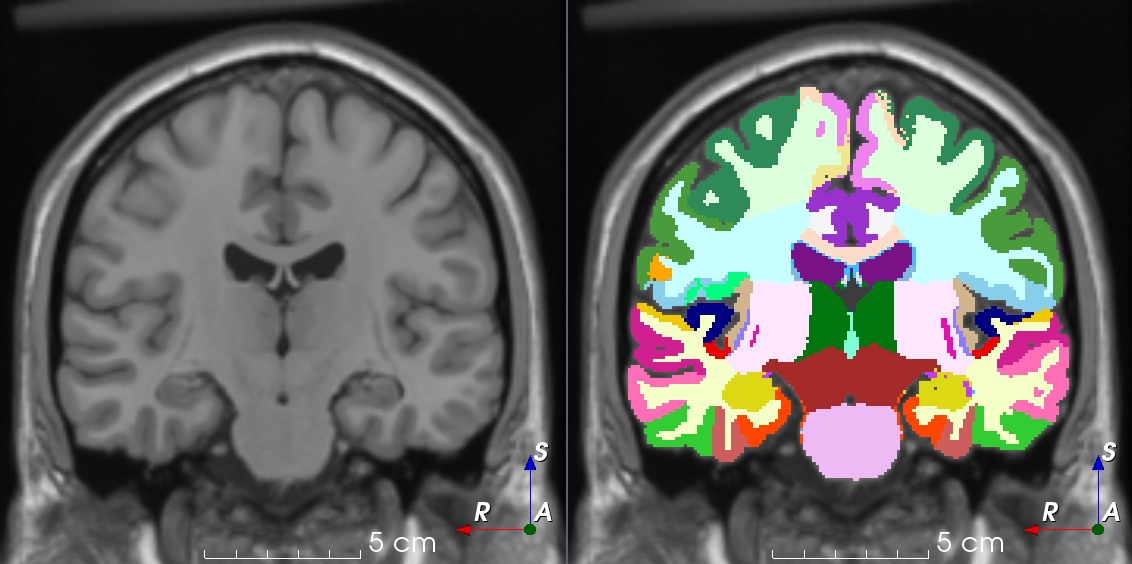
\includegraphics[width=0.8\textwidth]{Images/example_segmentation.png}
  \caption{Example of a multiclass semantic segmentation, different colors represent different classes}
  \label{fig:segmentation}
\end{figure}



% \section{Segmentation using Deep Neural Networks}
% As stated before, nowdays deep learning is the dominant method used for
% segmentation. Convolutional Neural Networks are still the most used type of
% networks used to date but new promising technique, as Graph Neural Networks or
% Transformers, are always more and more used.

% Chapter 2

\chapter{Segmentation Neural Networks}

\lhead{Chapter 2. \emph{Segmentation Neural Networks}} % This is for the header on each page - perhaps a shortened title
\label{chp:segmentation}
%----------------------------------------------------------------------------------------

\def\:{\hskip0pt} %Definisce un modo veloce per permettere a latex di sillabare correttamente anche parole come 4-connectivity. Il corretto utilizzo è il seguente: 4\:-\:connectivity.


\section{Supervised Learning}
In the medical image segmentation tasks, supervised learning is the most popular method, where the latest improvements mainly include network backbones, network blocks, and the design of novel loss functions.

\subsection{Backbone networks}
The encoder-decoder structure is the most popular end-to-end architecture, such as fully convolutional networks (FNC) like U-Net, Deeplab, and SegNet. The encoder part aims to extract high-level features from the input image and project them into a latent space. The decoder part instead restores the extracted features
from the latent space to the original space size.

\subsubsection{U-Net and V-Net}
In 2015, Ronneberger et al.
proposed U-Net which has been widely used for medical image segmentation and
many variants have been proposed also in recent years. The structure of U-Net
is symmetrical and the main scope is to fuse low-level features, which medical
images are usually noisy but show blurred boundaries, with high-level features
via skip connections.

U-Net was designed to deal with 2D images but when dealing with medical images,
we usually have to handle 3D images. A straightforward solution was to extract 2D
slices from the original image and fed them to the network and stack the outputs to
obtain the final 3D output.
The main drawback of this approach is that we lost the spatial information among
the slices as they are threatened as independent images. Motivated by this idea,
Çiçek et al. proposed a solution to this problem by using 3D convolutions inside
U-Net. This network, named 3D U-Net, includes only three down-sampling steps
because of the high computational cost of 3D Convolutions, leading to less
effective extraction of deep-layer image features.
Milletari et al. proposed a similar architecture, named V-Net, which employs more
skip connections than U-Net to design a deeper network.
Some Recurrent Neural Network mixed with U-Net has been proposed to model the
time dependence of image sequences.

\subsubsection{Recurrent Neural Networks}
Gao et al. joined LSTM and CNN to model the temporal relationships between
different brain MRI slices to improve segmentation accuracy. RNN can
capture local and global spatial features of images by considering the context
information
relationship. However, in medical image segmentation, the capture of complete
and valid temporal information requires good medical image quality (e.g. smaller
slice thickness and pixel spacing). Therefore, the design of RNN is uncommon for
improving the performance of medical image segmentation.

\subsubsection{Pseudo-3D Networks}
As stated before, most medical images are 3D images but using 3D
convolution requires a lot of computational resources. Therefore some pseudo-3D
segmentation methods have been proposed. For example, Vu et al. applied the
overlay of adjacent slices as input to the central slice prediction and then
fed the obtained 2D feature map into a standard 2D network.

\subsubsection{Generative Adversarial Networks}
\label{subsubsec:gan}
Another type of network that has been exploited in medical image segmentation is GAN, mostly for data augmentation by generating new samples. Pollastri et al. remodeled two different well-known GANs, Deep Convolutional GAN, and a Laplacian GAN, to generate both skin lesion images and their segmentation masks, making the augmentation process extremely straightforward.
In addition, the incorporation of prior knowledge about
organ shape and position may be crucial for improving the medical
image segmentation effect, where images are corrupted and
thus contain artifacts due to limitations of imaging techniques.
However, there are few works about how to incorporate prior
knowledge into CNN models. As one of the earliest studies in this field, Oktay et al. proposed a novel and general
method to combine a priori knowledge of shape and label
structure into the anatomically constrained neural networks
(ACNN) for medical image analysis tasks. In this way, the neural network training process can be constrained and guided to
make more anatomical and meaningful predictions, especially
in cases where input image data is not sufficiently informative or consistent enough (e.g., missing object boundaries).\\

After proposing U-Net, the encoder-decoder structure
became the most popular structure in medical image segmentation. The design of the network backbone focuses on more
efficient feature extraction in the encoder and feature recovery
and fusion in the decoder to improve segmentation accuracy.

\subsection{Network Function Block}
\subsubsection{Dense connection}
Dense connection is the most popular network block in medical image
segmentation, used to construct a kind of special convolution neural network. The
input of each layer comes from the output of all previous layers in the process of forwarding transmission. Inspired by this design, Guan et al. proposed an
improved U-Net by replacing each sub-block of the network with a form of dense
connection. Although the dense connection helps obtain richer image
features, it often reduces the robustness of feature representation to a certain
extent and increases the number of parameters.

\subsubsection{Inception block}
For CNNs, deep networks often give better performances than shallow ones, but they encounter some new problems such as vanishing gradient, high memory usage, and slow convergence. The inception structure used in GoogleNet overcomes these problems, and for this reason, it has been also used over medical images. Gu et al. proposed CE-Net by introducing the inception structure and atrous convolution to each parallel structure to extract features on a wide reception field. Such complex structure however leads to a difficult model modification.

\subsubsection{Depth separability}
To reduce the computational cost of 3D convolutions and their memory usage,
Howard et al. proposed MobileNet to decompose vanilla convolutions into
depthwise separable convolution and pointwise convolution.
% TODO: aggiungere calcolo del numero di calcoli fatti tra le 3D e le depth
% separable

\subsubsection{Attention}
\par
Attention block can selectively change input or assigns different weights to
input variables according to different importance.\\
\emph{Spatial Attention} block aims
to calculate the feature importance of each pixel in the space domain and extract
the key information of an image. Oktay et al. proposed attention U-Net, where
attention blocks were used to change the output of the encoder before fusing
features from the encoder and the corresponding decoder. The attention block
outputs a gating signal to control the feature importance of pixels at different
spatial positions.\\
Another type of attention block is the \emph{Channel attention},
which utilizes learned global information to emphasize selectively useful
features and suppress useless features. Hu et al. proposed SE-Net
introducing the channel attention to the field of image analysis and winning the
ImageNet Challenge in 2017.\\
Spatial and channel attention mechanisms are the two most popular strategies for
improving feature representation. However, spatial attention ignores the
difference between different channel information and treats each channel equally. On
the contrary, channel attention pools global information directly while
ignoring local information in each channel, which is a relatively rough
operation. Therefore, combining the advantages of two attention mechanisms,
researchers have designed many models based on a \emph{mixed domain attention block}.

\subsection{Loss functions}
In addition to improved segmentation speed and accuracy
by designing the network backbone and the function block, designing new loss
functions also resulted in improvements in subsequent inference-time
segmentation accuracy. Therefore,
a great deal of work has been reported on the design of
suitable loss functions for medical image segmentation tasks.

\subsubsection{Cross Entropy}
The cross-entropy loss has been the most popular loss function. It compares
pixel-wisely the predicted category vector with the real segmentation result
vector and is defined as:
$$
L_{CE} = -\sum_{i=1}^{N} \sum_{j=1}^{C} y_{ij} \log \hat{y}_{ij}
$$
where $y_{ij}$ is the real segmentation result vector, $\hat{y}_{ij}$ is the
predicted segmentation result vector, $n$ is the number of pixels in the image,
and $C$ is the number of categories. The cross-entropy loss is easy to
implement and has been widely used in medical image segmentation tasks. However,
it is not suitable for segmentation tasks with imbalanced data, because it does
not consider the class imbalance problem. Therefore, a \emph{weighted cross
entropy loss} and \emph{balanced cross entropy} have been proposed to solve this
problem, where a $\beta$ hyperparameters are added to the loss function to adjust
the weight of each class.

\subsubsection{Dice Loss}
The Dice coefficient is a popular metric for the evaluation of medical image
segmentation tasks. This metric is the measure of overlap between a segmentation
result and its corresponding ground truth:
$$
DSC = \frac{2 \times |A \cap B|}{|A| + |B|}
$$
where $A$ and $B$ are the segmentation result and the ground truth,
respectively. The \emph{Dice Loss} is then formulated as follows:
$$
L_{DSC} = 1 - \frac{2 \times y \times \hat{y} + 1}{y + \hat{y} + 1}
$$
Here 1 is added to the denominator to avoid the division by zero in the edge
case when both $y$ and $\hat{y}$ are zero. The Dice loss is a good choice even
for uneven samples, however, it easily influences the backpropagation and leads
  to a training difficulty.

\subsubsection{Generalized Dice Loss}
Although Dice Loss can solve the problem of class imbalance to a certain extent,
it does not work for serious class imbalance. To solve this problem, researchers
have proposed a \emph{Generalized Dice Loss} that can be used for both binary
and multi-class segmentation tasks. The generalized Dice loss is defined as:
$$
L_{GDSC} = 1 - \frac{1}{m}\frac{2\sum_{j=1}^{m} \omega_j
\sum_{i=1}^{n}y_{ij}\hat{y}_{ij}}{\sum_{j=1}^{m}\omega_j\sum_{i=1}^{n}(y_{ij} +
\hat{y}_{ij})}
$$
where the weight $\omega_j$ is used to adjust the weight of each class, and $\omega_j = 1/(\sum_{i=1}^{n}p_{ij})^2$.

\subsubsection{Boundary Loss}
Another approach that solves the problem of class imbalance has been proposed by
Kervadec et al. for the task of brain lesion segmentation. They proposed a Boundary Loss which aims to minimize the distance between segmented boundaries
and labeled boundaries. Results show that the combination of the Dice loss and
the boundary loss is superior to the single ones. The composite loss is defined
as:
$$
L = \alpha L_{DSC} + (1 - \alpha) L_{B}
$$
where the Boundary Loss $L_{B}$ for a binary segmentation is defined as:
$$
L_{B} = \sum \phi(y) \times \hat{y}
$$
where $\phi(y)$ is the signed distance function applied to the real segmentation $y$.

\par
For medical image segmentation, the improvement of loss mainly focuses on the
problem of segmentation of small objects in a large background (the problem of
class imbalance). Chen et al. proposed a new loss function by applying
traditional active contour energy minimization to convolutional neural networks,
Li et al. proposed a new regularization term to improve the cross-entropy loss
function, and Karimi et al. proposed a loss function based on Hausdorff
distance (HD). Besides, there is still a lot of work trying to deal with this
problem by adding penalties to lose functions or changing the optimization
strategy according to specific tasks.\\
In many medical image segmentation tasks, there are often only one or two
targets in an image, and the pixel ratio of targets is sometimes small, which
makes network training difficult. Therefore, to improve network training and
segmentation accuracy, it is easier to focus on smaller targets by changing loss
functions than to change the network structure. However, the design of loss
functions is highly task-specific, so we need to analyze carefully task
requirements, and then design reasonable and available loss functions.

\section{Weakly Supervised and Unsupervised Segmentation}
Although convolutional neural networks show goods performances for medical
image segmentation, results seriously depend on high-quality
labels. It is rare to build many datasets with many high-quality labels,
especially in the field of medical image analysis, since data acquisition and
labeling often incur high costs. Therefore, a lot of studies on incomplete or
imperfect datasets are reported. Unsupervised learning is a very important approach that improves the performance of medical image segmentation. In this
section, we will introduce weakly supervised learning, a method that makes
use of unsupervised learning for unlabelled data in combination with supervised
learning with labeled data.

\subsection{Data Augmentation}
Performing data augmentation is mandatory in absence of a largely labeled dataset, and is still considered good practice even when we have enough data. However, new data generated with this method produce images that are highly correlated with the original images.

\subsubsection{Traditional methods}
With traditional methods, we refer to all the computer vision techniques such as adding/removing noise, changing brightness, saturation, contrast, colors, and changing the image layout with rotations, distortion, scaling, etc. These techniques are still very used today, usually combining them together with random parameters. Some of these algorithms may require a non-negligible computational cost thus usually performed before the training procedure.

\subsubsection{Conditional Generative Adversarial Networks}
As already described in Section \ref{subsubsec:gan}, GAN and its variants have been widely for data augmentation. In particular, cGANs are often used in combination with standard GANs to generate labels relative to a given synthetic image.

\subsection{Transfer Learning}
Pre-trained model parameters are often used to initialize a new model,
transfer learning can achieve fast training for data with limited labels. The
most popular approach is to use a model pretrained on ImageNet before performing
the training on the medical data. Experiments demonstrated that this approach is
useful as it improves the accuracy of segmentations. However, domain
adaptation may be a problem when applying models trained over natural images to
medical image analysis tasks. Moreover, these methods are hardly applicable to
3D medical image analysis because such pre-trained models rely on 2D datasets.\\
Hatamizadeh et al. recently proposed an unsupervised approach to pre-train a
given model by relying only on unannotated medical images of the same domain of
the main tasks. In practice, the network is trained to perform a variety of tasks
such as image reconstruction, classification of the rotation applied to the
original image, etc. which can be performed in an unsupervised manner. Later,
these tasks heads of the network are detached and the training on the main task
is performed. Such pretraining aims to train the network to learn how to extract
high-level features from a specific type of medical images, such as CT or MRI.\\
Also, Cipriano et al. recently proposed a pre-training approach based on sparse labels.
This type of labels are way easier to obtain but is not as accurate as the real dense labels. They fed these labels to the network together with the input
image for a given number of steps, then used the learned parameters to train the
network to produce the segmentation by relying only on the input, without the
sparse labels.


\section{Current direction of research}
Until now we described the most popular network structures and loss functions
for medical image segmentation tasks that were proposed and used up to date.
Since the rise in the popularity of vision transformers and graph neural networks,
some novelty architectures are being proposed in medical imaging. Results
obtained are still not as good as those obtained with traditional architectures,
aside from some really specific tasks or datasets, but they are still interesting and
promising.\\

\subsection{Network Architecture Search}
The design process of network architecture is a very time-consuming task, and
it is often difficult to find the best architecture for a given task. Therefore,
many researchers have proposed methods to automate the design of network
architectures. Such methods, named NAS (Network Architecture Search), focus on
the \emph{search space}, \emph{search strategy}, and \emph{performance
estimation}.
The search space is a candidate collection of network structures to be searched.
The search space is divided into a global search space that represents the
search for the entire network structure, and a cell-based search space that
searches only a few small structures that are assembled into a complete large network by the ways of stacking and stitching. The search strategy aims to find
the optimal network structure as fast as possible in search spaces. Popular
search strategies are often grouped into three categories, reinforcement-based
learning, evolutionary algorithms, and gradients. The performance estimation
strategy is the process of assessing how well the network structure performs on
target datasets. For NAS techniques, researchers pay more attention to the
improvement of search strategies since search space and performance estimation
methods are usually rarely changed.\\
Isensee et al. argued that too much manual adjustment on network structure could
lead to over-fitting for a given dataset, and therefore proposed a medical image
segmentation framework no-newUNet (nnU-Net) that adapts itself to any new
dataset. The nnUNet automatically adjusts all hyperparameters according to the
properties of the given dataset without manual intervention. Therefore, the
nnU-Net only relies on vanilla 2D UNet, 3D UNet, UNet cascade, and a robust
training scheme. It focuses on the stage of pre-processing (resampling and
normalization), training (loss, optimizer settings, data augmentation),
inference (patch-based strategies, test-time-augmentations integration, model
integration, etc.), and post-processing (e.g., enhanced single pass domain). In
practical applications, the improvements in network structure design usually
depend on experiences without adequate interpretability theory support,
Moreover, more complex network models indicate a higher risk of over-fitting.


\subsection{Graph Convolutional Neural Network}
Graph Convolutional Neural Network (GCN) is a type of neural network that
utilizes graph structure to process data. In practice, the Euclidean space of the
image can be converted into graphs that can be modeled using GCN.

Gao et al. designed a new graph pooling (gPool) and graph unpooling (gUnpool)
operation based on GCN and proposed an encoder-decoder model namely graph U-Net.
The graph U-Net achieves better performance than popular UNets by adding a small
number of parameters. In contrast to traditional convolutional neural networks
where deeper is better, the performance of the graph U-Net cannot be improved by
increasing the depth of networks when the value of depth exceeds 4. However, the
graph U-Net shows a stronger capability of feature encoding than popular U-Nets
when the value of depth is smaller or equivalent to 4.

Yang et al. proposed the end-to-end conditional partial residual plot
convolutional network CPR-GCN for automatic anatomical marking of coronary
arteries. Authors showed that the GCN-based approach provided better performance
and stronger robustness than traditional and recent depth learning-based
approaches. Results from these GCNs in medical image segmentations are
promising, as the graph structure has high data representation efficiency and
a strong capability of feature encoding.

\subsection{Interpretable Shape Attentive Neural Network}
Currently, many deep learning algorithms tend to make judgments by using
"memorized`` models that approximately fit input data. As a result, these
algorithms cannot be explained sufficiently and give convincing evidence for
each specific prediction. Therefore, the study of the interpretability of deep
neural networks is a hot topic at present. Sun et al. proposed the SAU-Net which
focuses on the interpretability and robustness of models. The proposed
architecture attempts to address the problem of poor edge segmentation accuracy
in medical images by using a secondary shape stream. Especially, the shape stream
and the regular texture stream can capture rich shape-dependent information in
parallel. Furthermore, both spatial and channel attention mechanisms are used for
the decoder to explain the learning capability of models at each resolution of
U-Net. Finally, by extracting the learned shape and spatial attention maps, we
can interpret the highly activated regions of each decoder block. The learned
shape maps can be used to infer the correct shapes of interesting categories learned
by the model. The SAU-Net can learn robust shape features of objects via
the gated shape stream and is also more interpretable than previous works via
built-in saliency maps using attention.

\subsection{Vision Transformer}
Recently, transformer-based architectures have become very popular and replaced the convolutional operator and use self-attention modules to compose entire
encoderdecoder structures that can encode long-range dependencies.
It has been a great success in the field of natural language processing.
Dosovitskiy et al. proposed Vision Transformer (ViT) that can classify
images directly using the Transformer.
Recently, a large number of researchers have applied the transformer to medical
image segmentation. CNNs have a comparative advantage in extracting the
underlying features. These low-level features form the key points, lines, and
some basic image structures at the patch level. However, when we detect these
basic visual elements, the higher-level visual semantic information is often
more concerned with how these elements relate to each other to form an object,
and how the spatial location of objects relates to each other to form the scene.
At present, the transformer is more natural and effective in dealing with the
relationships between these elements. However, if all the convolutional
operators in CV tasks are replaced by Transformer, it may suffer from many
problems, such as high computational cost and memory usage. From existing research, the combination of Transformer and CNNs may lead to better results.
Recently, Chen et al. proposed a U-Net shaped network, where the encoder was
made of ViT only while the decoder was fully convolutional.


% Chapter 3

\chapter{The Maxillo Dataset}

\lhead{Chapter 3. \emph{The Maxillo Dataset}} % This is for the header on each page - perhaps a shortened title
\label{chp:maxillo}
%----------------------------------------------------------------------------------------

\def\:{\hskip0pt} %Definisce un modo veloce per permettere a latex di sillabare correttamente anche parole come 4-connectivity. Il corretto utilizzo è il seguente: 4\:-\:connectivity.

\section{Introduction}
Nowadays, perfect anatomical annotation accuracy is usually not achieved, in
favor of a fast execution time. A sparse annotation (Fig. \ref{fig:2dannot}),
performed on a 2D image, can be realized in a relatively small amount of time,
and has become the de facto standard in radiologic medical centers for dentistry
and maxillofacial purposes (a specialty also known as dento-maxillofacial
radiology). However, 2D annotations lack a considerable amount of inner
information about the bone structure and the IAN position. Surgeons rely on a
partial and incomplete idea of nerve positioning, which is generally sufficient
for a positive outcome of surgical intervention but does not represent an
accurate anatomical representation. Switching to 3D annotations (Fig.
\ref{fig:3dannot}) solves the issue, but raises the costs in terms of working
time: the manual segmentation of a single scan volume, depending on the
available software, can take hours. Therefore, although dento-maxillofacial
radiology would largely benefit from 3D annotated patients, any manual method
currently appears unsuitable for practical applications.

\begin{figure}
  \centering
  \begin{subfigure}{.35\textwidth}
    \centering
    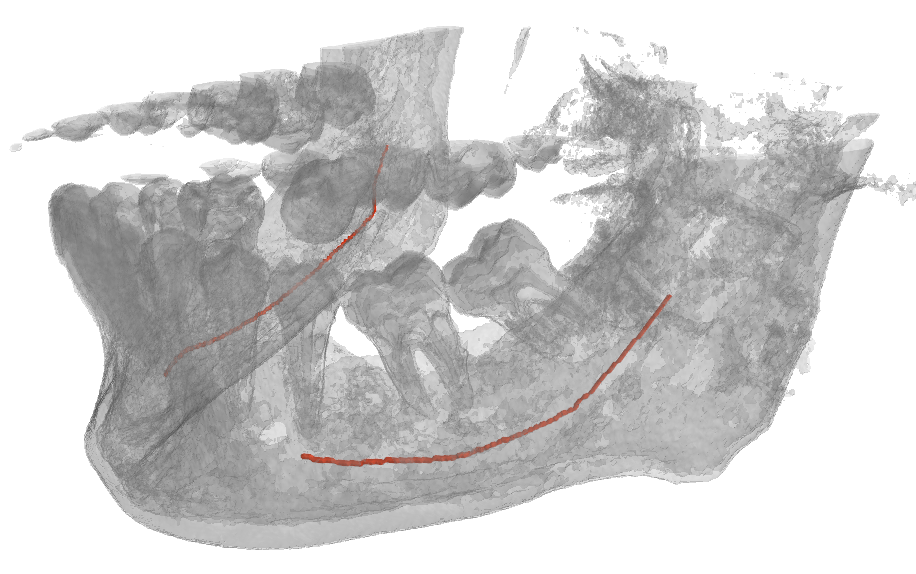
\includegraphics[width=\textwidth]{Images/sparse_annotation.png}
    \caption{2D annotation.}
    \label{fig:2dannot}
  \end{subfigure}
  \begin{subfigure}{0.35\textwidth}
    \centering
    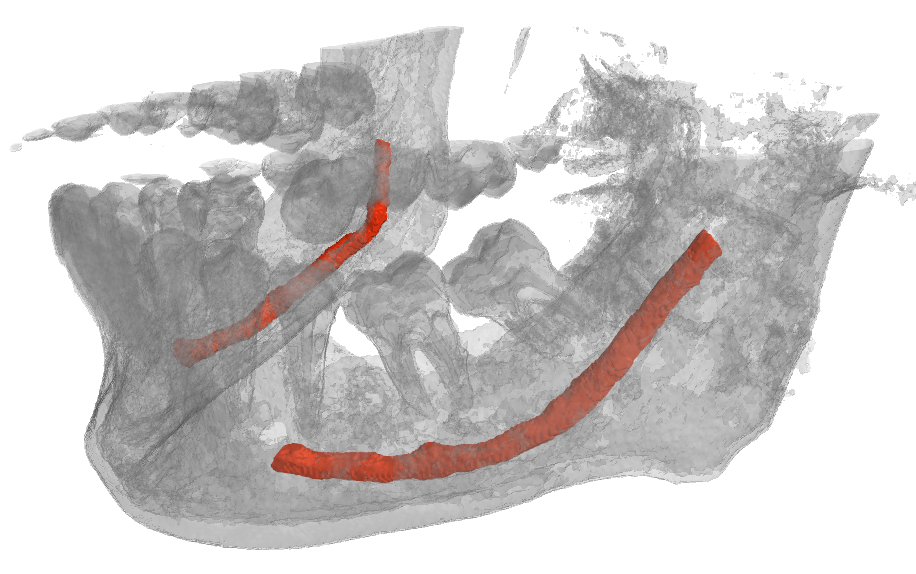
\includegraphics[width=\textwidth]{Images/dense_annotation.png}
    \caption{3D annotation.}
    \label{fig:3dannot}
  \end{subfigure}
  \caption{2D and 3D annotations of the same patient.}
  \label{fig:2d3dannot}
\end{figure}

An additional constraint when dealing with the medical branch of deep learning
regards the extra consideration for sensitive data, which must always be taken
into account. Medical data contain a huge amount of personal information which
must be protected through data anonymization. Besides the sensible details about
the patient, generally stored in the DICOM format, when it comes to medical
imaging, the personal features of one subject can be inherently carried by the
images. Therefore, in order to evaluate the correctness of the anonymization
steps and the security of the information, every medical dataset must undergo
evaluation of specific committees. Several bureaucratic steps generally stand
before the official release to the scientific community. This circumstance,
combined with the laws of individual countries, creates a serious burden for the
spread of medical datasets and makes any contribution valuable. For those
reasons, deep learning works applied to medical imaging — and in particular, to
the maxillofacial field— are often based on private internal datasets. Despite
any alleged intention, datasets are rarely released after publication, creating
a vast information gap for the research community: researchers are unable to
replicate experiments and lack valid benchmarks for their novelties.

\section{Dataset}
Cipriano et al. \cite{cipriano2022deep} have released a public dataset of
maxillofacial scans with a sparse and deep labels, which is the first of its
kind.
The 3D CBCT volumes composing the dataset have been acquired by the Affidea
center located in Modena, Italy. Affidea is a leading pan-European healthcare
group specialized in the provision of advanced diagnostics, specialist
outpatient services, laboratory analyses, physiotherapy and rehabilitation,
cancer diagnosis, and treatment. It counts $312$ different centers in $15$
different countries, with about 11 000 professionals. The dataset counts $347$
dental scans obtained by means of Cone Beam Computed Tomography
(\texttt{NewTom/NTVGiMK4, 3 mA, 110 kV, 0.3 mm cubic voxels}). Pixel spacing and
intra-slice distance are always $0.3$ millimeters. Data volumes are already
converted to the Hounsfield Unit (HU) and their values range between $-1000$ and
$5264$. During the conversion to HU we also took care of the proper processing
for the window width and center according to the DICOM format. Volume shapes
range from $(148, 265, 312)$ to $(178, 423, 463)$ for the \texttt{Z}, \texttt{Y}
and \texttt{X} axes respectively. Every patient was anonymized, hence we were
only able to access a few personal details - namely gender, age, and year of the
scan. Specifically, 59\% of the patients are female, all the scans were
performed between 2019 and 2020, and volumes belong to patients with ages in the
range $(10-100]$ with the highest frequencies in ranges $(20-30]$ and $(60-70]$.

\subsection{2D sparse annotations}
Technicians involved in the diagnostic exam were also responsible for the
original sparse annotation of the mandibular canal. This annotation performed on
2D panoramic views of the jawbone is employed in everyday surgical practice to
measure the height and depth of the sites where the implant must be placed,
avoiding inferior alveolar nerve injuries. In these labels, the upper bound of
the canal is marked along the entire dental arch, providing a useful sparse
approximation trace of nerve position. Particularly, the annotation process
starts from an axial slice (Fig. \ref{fig:axial-slice} of the original volume.
Upon this slice, a spline is manually drawn to fit the central part of the
jawbone.

\begin{figure}[ht]
  \centering
  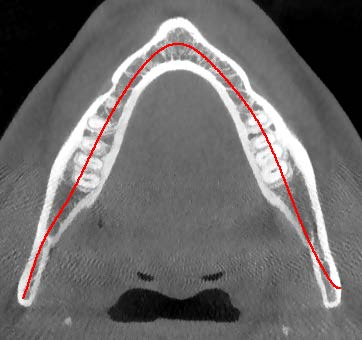
\includegraphics[width=0.45\textwidth]{Images/axial-slice.jpg}
  \caption{Axial slice.}
  \label{fig:axial-slice}
\end{figure}

This spline, called the panoramic base curve, is then employed for generating
the panoramic view (Fig. \ref{fig:panoramic}) composed by the voxels of the
curved plane identified by the base curve and orthogonal to the axial slice.
From this view, the inferior alveolar nerve canal should be clearly identifiable
and can be annotated as in Fig. \ref{fig:panoramic_annotated}.

\begin{figure}[!ht]
  \centering
  \begin{subfigure}{0.8\textwidth}
    \centering
    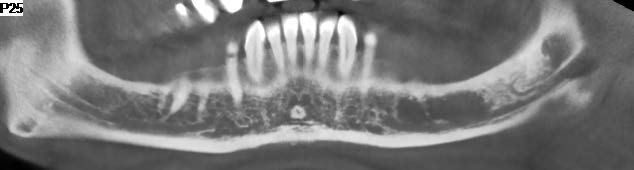
\includegraphics[width=\textwidth]{Images/panoramic.jpg}
    \caption{Panoramic view obtained from the spline drawn on the axial slice.}
    \label{fig:panoramic}
  \end{subfigure}

  \begin{subfigure}{0.8\textwidth}
    \centering
    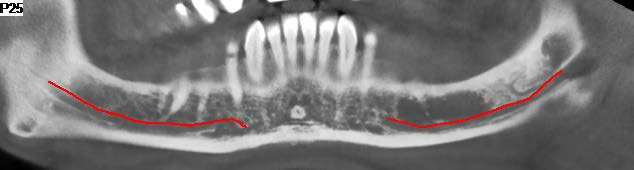
\includegraphics[width=\textwidth]{Images/panoramic_annotated.jpg}
    \caption{Panoramic view with the inferior alveolar nerve canal annotated in
    red.}
    \label{fig:panoramic_annotated}
  \end{subfigure}
  \caption{Panoramic view and its annotation.}
  \label{fig:2d3dannot}
\end{figure}

\subsection{3D dense annotations}
In order to obtain finely-grained annotations, a team of doctors with years of
experience in maxillofacial surgery elaborated $91$ volumes to produce dense
voxel-level annotations of the canal. The proposed dataset of $347$ scans is
therefore divided into two partitions: the primary dataset, composed of the $91$
volumes for which both dense and sparse annotations are available, and the
secondary dataset, only sparsely annotated.

The entire voxel-level annotation procedure has been performed by means of a
tool developed by Mercadante et al. \cite{mercadante2021cone} which allowed to
drastically reduce the burden necessary to produce the 3D label.
The annotation steps can be summarized as follows:
\begin{enumerate}
  \item{After loading the input data, the arch approximation that better
    describes the canal course is identified inside one of the axial images and
    manually adjusted. The output is a one-pixel thick curve crossing the dental
    arch which is approximated with a polynomial. The result is similar to the
    one in Fig. \ref{fig:axial-slice}, but this time it is automatically
    generated and manually adjusted only if needed.}

  \item{Sampling the polynomial, the tool thus generates a Catmull-Rom spline.
    For each point of the spline, a perpendicular line (lying on the axial
    plane) is computed (Fig. \ref{fig:csl}). These lines are called
    Cross-Sectional Lines or CSLs in short. Here, a different resolution of the
    spline generates more or fewer CSLs. This represents a crucial step for
    having a complete annotation of the mandibular canal. Indeed, with a short
    spline, some regions of the jawbone, especially near the mandibular foramen,
    would be excluded from the next stages.}

  \item{CSLs are the base of Multi Planar Reformations(MPRs) called
    Cross-Sectional Views (CSVs). These views are 2D images obtained
    interpolating the values of the respective baselines (CSL) across the whole
    volume height. As an example, the blue plane reported in Fig.
    \ref{fig:csl-orthogonal} is a Cross-Sectional Plane (CSP) generating a
    cross-sectional View. CSPs are additionally rotated around the CSLs, to have
    CSVs orthogonal to the canal slope.}

  %TODO Fig 6
  \item{For each CSV, a closed Catmull-Rom spline is finally drawn to annotate
    the position of the IAC (green lines of Fig. 6).}

  \item{The splines are saved as the coordinates of their control points. The
    final smooth and precise ground-truth volume constituting the dataset is
    generated from this set of points by means of the \textalpha-shape algorithm
    \cite{edelsbrunner1983shape}, which is described in detail in the Section
    \ref{sec:alpha}.}
\end{enumerate}

\begin{figure}[!ht]
  \centering
  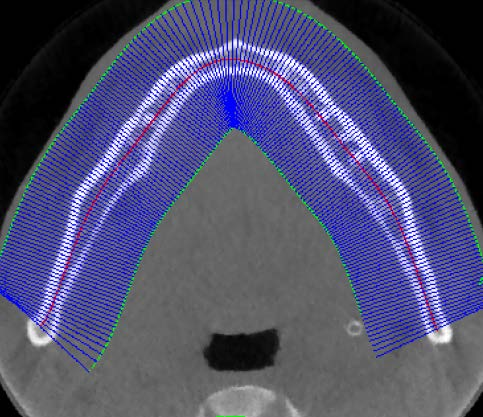
\includegraphics[width=0.45\textwidth]{Images/csl.jpg}
  \caption{Cross-Sectional Lines.}
  \label{fig:csl}
\end{figure}

\begin{figure}[!ht]
  \centering
  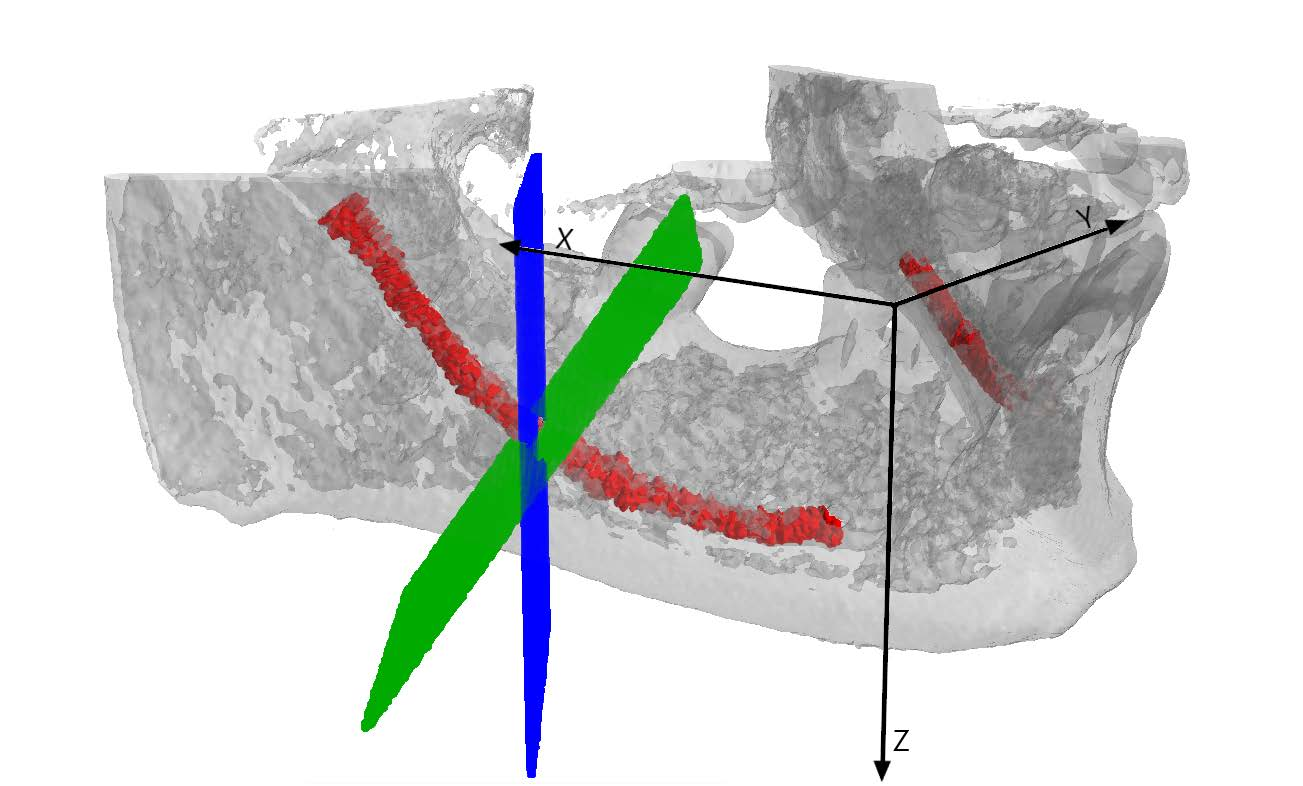
\includegraphics[width=0.5\textwidth]{Images/csl-orthogonal.jpg}
  \caption{Cross-Sectional Lines.}
  \label{fig:csl-orthogonal}
\end{figure}

Comparing the two procedures, it is possible to see that while sparse
annotations are quick and easy to obtain, creating dense labels from 3D volumes
is a very tedious and time-consuming process. For this reason, researchers
typically have few dense annotations available and preserve them as the test
set. Indeed, densely annotated volumes must always be used in tests, to ensure a
real medical feedback on model performance.

\subsection{Pre-processing with \textalpha-shape}
\label{sec:alpha}
The hand-drawn ground truth annotations produced with the tool described in the
previous section result in a dense and jagged point set; an example is depicted
in Fig. \ref{fig:pointset}. Starting from this point set, we reconstruct a
smoother polygon mesh in the form of the \textalpha-shape. The \textalpha-shape,
defined by Edelsbrunner et al. is a generalization of the concept of the convex
hull, useful to capture the intuitive notion of the shape of a point set. The
definition refers to the 2-dimensional case, but the extension to point sets in
$k$ dimensions is straightforward. The \textalpha-shape is parameterized over
$\alpha \in \mathbb{R}$, which determines the "crudeness`` of the result.\\

\begin{figure}[t]
  \centering
  \begin{subfigure}{.45\textwidth}
    \centering
    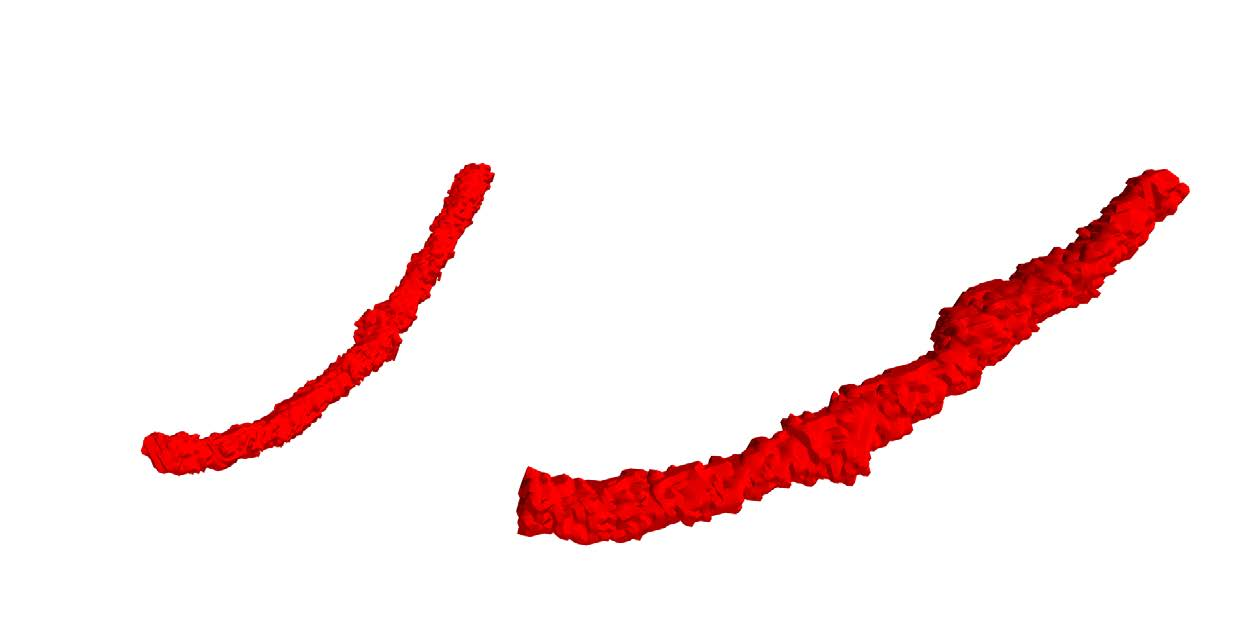
\includegraphics[width=\textwidth]{Images/pointset.jpg}
    \caption{Jagged point set.}
    \label{fig:pointset}
  \end{subfigure}
  \begin{subfigure}{0.45\textwidth}
    \centering
    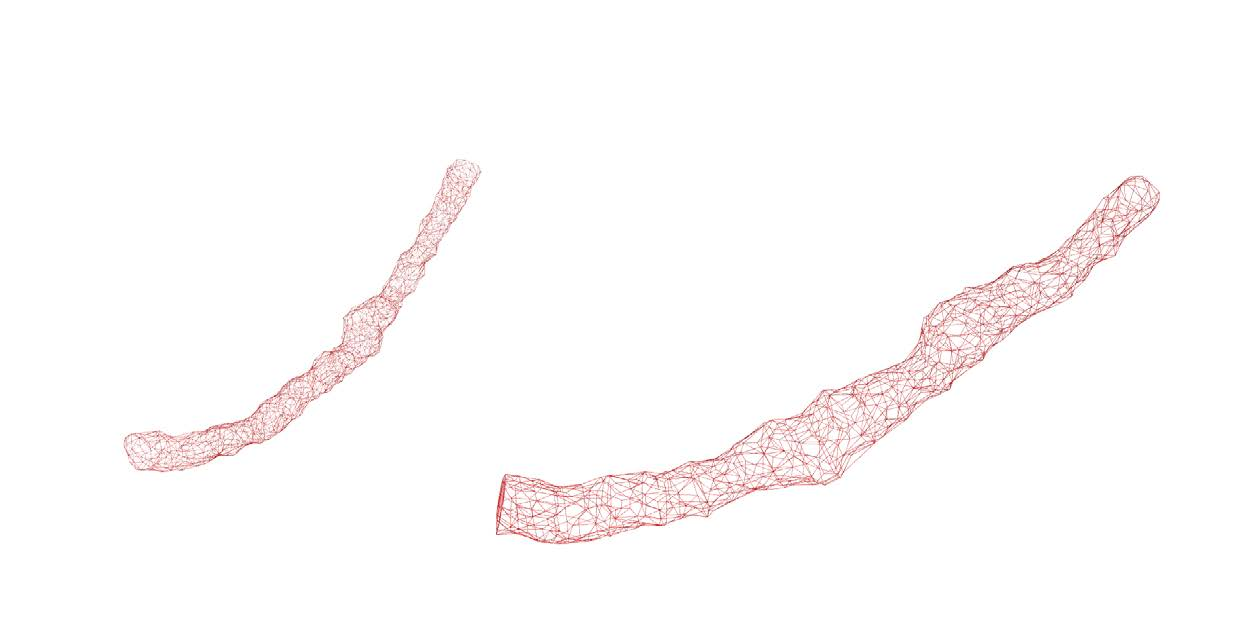
\includegraphics[width=\textwidth]{Images/alpha1.jpg}
    \caption{\textalpha-shape mesh.}
    \label{fig:alpha1}
  \end{subfigure}
  \begin{subfigure}{0.45\textwidth}
    \centering
    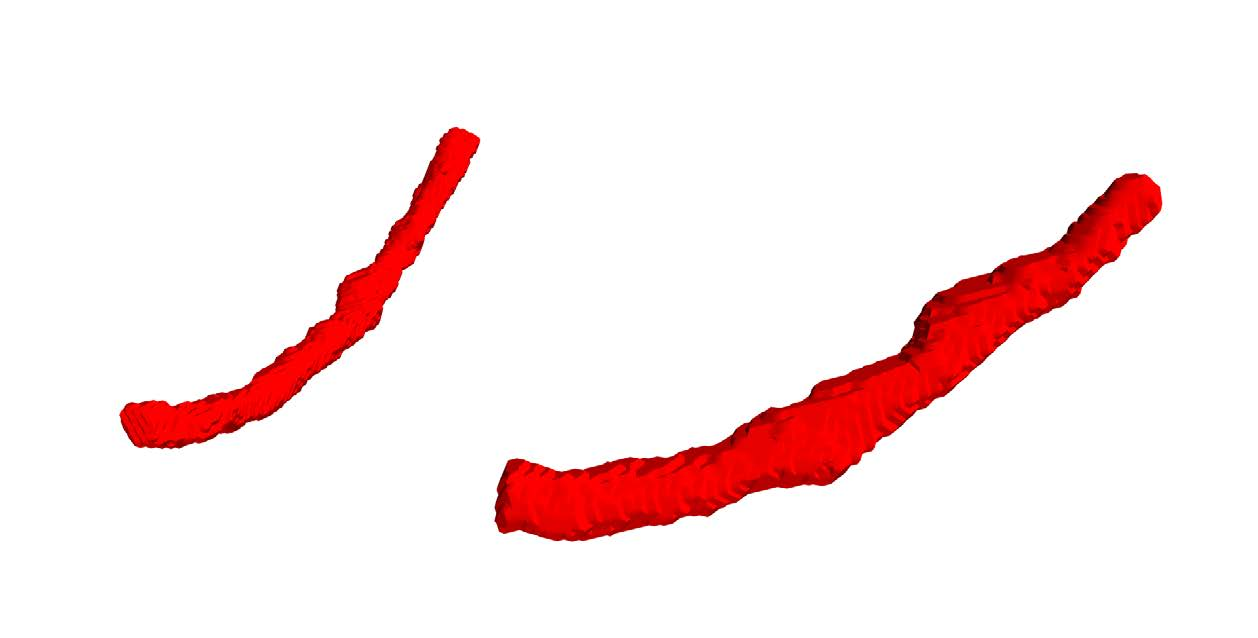
\includegraphics[width=\textwidth]{Images/alpha2.jpg}
    \caption{Voxelized raster volume.}
    \label{fig:alpha2}
  \end{subfigure}
  \caption{The annotation tool outputs a dense and jagged point set (a), which
  shape is given by the concave \textalpha-shape (b). Finally, the obtained
  polygonal mesh undergoes voxelization, resulting in a binary raster volume (c)
  that is used as ground truth for the training process.}
  \label{fig:preprocessing}
\end{figure}

First, a generalized disk of radius $\frac{1}{\alpha}$, named $D_\alpha$, is
defined as:
$$
D_\alpha=
\begin{cases}
  \text{The complement of a disc of radius} -\frac{1}{\alpha}, & \text{if $\alpha<0$}\\
  \text{A halfplane} & \text{if $\alpha=0$}\\
  \text{A disc of radius} \frac{1}{\alpha}, & \text{if $\alpha>0$}\\
\end{cases}
$$
Then, given a point set $\mathcal{S}$ and a specific value for \textalpha, the
\textalpha-shape graph is constructed in the following way: an edge is
created between two points $p_i$ and $p_j$ whenever there exists
a $D_\alpha$ containing the entire $\mathcal{S}$, and which has the property
that $p_i$ and $p_j$ lie on its boundary. It is straightforward to
notice that, when $\alpha = 0$, this process constructs the convex
hull. Instead, positive or negative values of \textalpha\;allow building
cruder or finer shapes respectively, with the latter possibly including concave
angles. Because of the geometrical nature of the alveolar nerve, we are indeed
exclusively interested in concave \textalpha-shapes, i.e., with $\alpha < 0$.
When $\alpha < 0$, the \textalpha-shape can be computed starting from the
Delaunay triangulation: the set of triangles of the Delaunay triangulation whose
circumradius is at most $\frac{1}{\alpha}$ form a simplicial subcomplex, called
\textalpha-complex, and its border coincides with the \textalpha-shape.
The process is exemplified in Fig. \ref{fig:alphabuild}.

The generalization of the above notions to $3$ dimensions is just a matter of
substituting disks and triangles with spheres and tetrahedra. An example of
\textalpha-shape constructed from the volumetric annotations of the alveolar
nerve is depicted in Fig. \ref{fig:alpha1}.
\begin{figure}[h!]
  \centering
  %%%%%%%%%%%%%%%%
  \begin{subfigure}{1\textwidth}
    \centering
    \begin{subfigure}{0.24\textwidth}
      \centering
      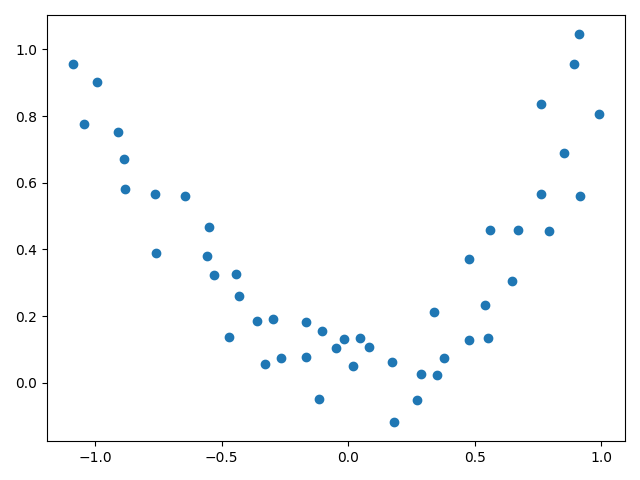
\includegraphics[width=\textwidth]{Images/alpha_1.png}
      \caption{Point set}
      \label{fig:pointset}
    \end{subfigure}
    %%%%%%%%%%%%%%%%
    \begin{subfigure}{0.24\textwidth}
      \centering
      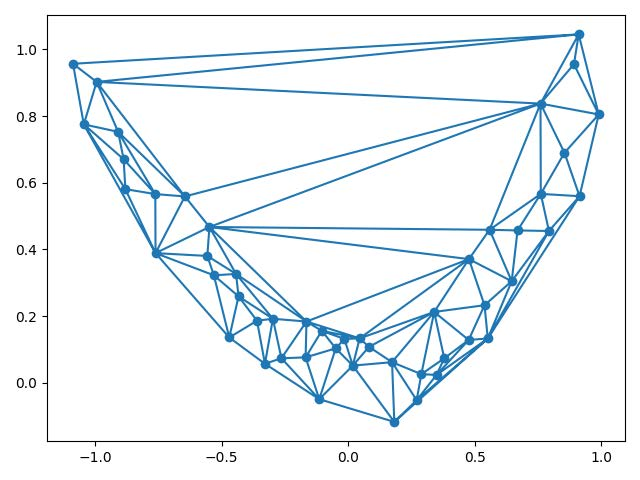
\includegraphics[width=\textwidth]{Images/alpha_2.jpg}
      \caption{Delunay}
      \label{fig:delunay}
    \end{subfigure}
    %%%%%%%%%%%%%%%%
    \begin{subfigure}{0.24\textwidth}
      \centering
      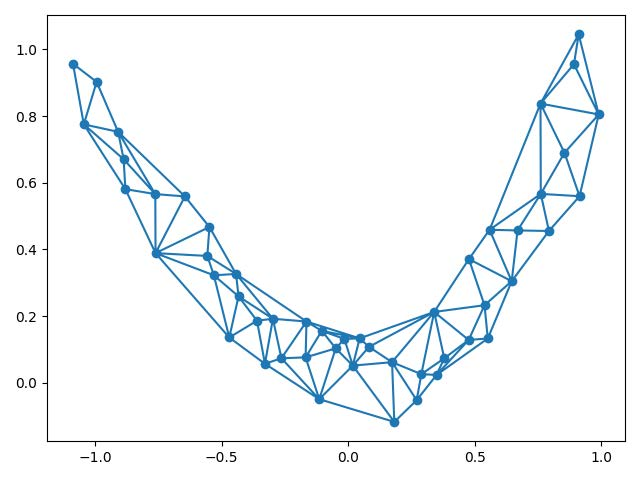
\includegraphics[width=\textwidth]{Images/alpha_3.jpg}
      \caption{\textalpha-complex}
      \label{fig:alphacomplex}
    \end{subfigure}
    %%%%%%%%%%%%%%%%
    \begin{subfigure}{0.24\textwidth}
      \centering
      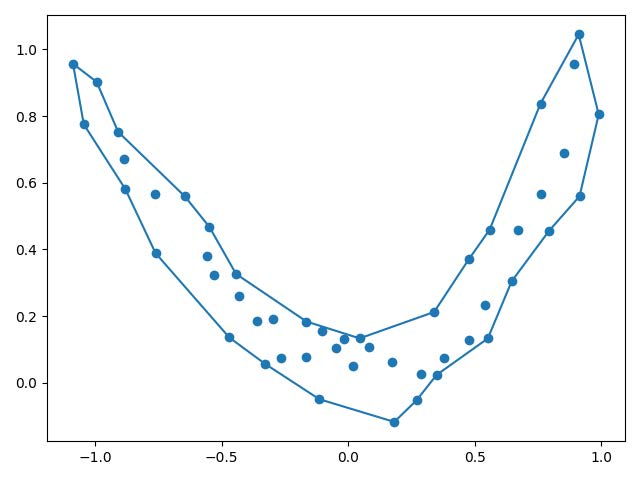
\includegraphics[width=\textwidth]{Images/alpha_4.jpg}
      \caption{\textalpha-shape}
      \label{fig:alphashape}
    \end{subfigure}
  \end{subfigure}
  %%%%%%%%%%%%%%%%
  \caption{\textalpha-shape construction process for the point set of
  \ref{fig:pointset}, with $\alpha = -2.5$. First the Delaunay triangulation is
  built \ref{fig:delunay}, then only triangles whose circumradius is at most
  $-\frac{1}{\alpha}$ are kept, which form a subcomplex called
  \textalpha-complex \ref{fig:alphacomplex}. Finally, the border of the
  \textalpha-complex is the \textalpha-shape \ref{fig:alphashape}.}
  \label{fig:alphabuild}
\end{figure}

The \textalpha-shape is a good representation of the annotated volume, but
because it is a polygonal mesh, it cannot directly be used as a ground truth
segmentation mask for training a neural network. Therefore, the next mandatory
step is voxelization, through which the \textalpha-shape is transformed into
a binary raster volume. The voxelization of a polygonal mesh consists of finding
which cubes (voxels) of a 3-dimensional grid intersect any triangle composing
the mesh: the specific method used to check triangle-cube intersection has been
developed by Voorhies. The final result of the ground truth preprocessing is
illustrated in Fig. \ref{fig:alpha2}.


% Chapter 4

\chapter{Code Refactoring}

\lhead{Chapter 4. \emph{Code Refactoring}} % This is for the header on each page - perhaps a shortened title
\label{chp:refwork}
%----------------------------------------------------------------------------------------

\def\:{\hskip0pt} %Definisce un modo veloce per permettere a latex di sillabare correttamente anche parole come 4-connectivity. Il corretto utilizzo è il seguente: 4\:-\:connectivity.
\section{Introduction}
Cipriano et al. spent some effort developing the dataset and a to design a
network which was capable to perform the segmentation of the Inferior Alveolar
Canal.
Together with the novel dataset, they proposed a modified version of
U-Net 3D as a backbone for both the label propagation and the IAC segmentation.
Both these networks and methods were introduced in the previous
chapters and will be explained more in detail in the following sections.
As the code was written near the deadline for the submission of the paper,
the authors did not have focused on producing a codebase that was optimized for
reusability, extensibility, and efficiency.
For this reason, my work starts by refactoring the codebase to add these features
which improved all my successive experiments.

\section{Reference Work}
The reference work that has been taken as starting point for this work has been
made by Cipriano et al. in 2022 \cite{cipriano2022improving}.
The pipeline proposed can be divided into two main steps: the deep label
propagation and the IAC segmentation.

\subsection{Positional PadUNet3D}
A slightly modified version of 3D U-Net has been proposed as a backbone for both
steps. Differently from the original 3D U-Net architecture, every
three-dimensional convolution in our CNN applies 2 pixels padding along each
dimension. Although this alteration does not cause any variation in terms of
performance, it ensures that the output of each convolution has the same size as
its input along axis \emph{x}, \emph{y}, and \emph{z}.

Resolution changes are therefore due uniquely to the three max-pooling layers,
each halving the size of the volumes. When using the aforementioned input size,
the encoder output is composed of $512$ feature maps of size $10 \times 10
\times 10$. Inside the decoder, on the other hand, resolution changes are caused
by transposed convolutions, with dimensions $2 \times 2 \times 2$ for both the
kernel and stride to double the size of the feature maps. This adjustment
ensures resolution symmetry between features in the decoder and corresponding
maps in the encoder, thus allowing them to be simply concatenated with skip
connections. Moreover, the output of the model naturally has the same dimensions
as the input. The final output is a single channel volume, to which we apply a
Sigmoid activation function and a threshold at $0.5$ to obtain the final binary
prediction mask.

The segmentation architecture is further enriched with a positional embedding.
Since our sub-volumes are extracted from the original scan following a fixed
grid, we exploit positional information derived from the location of the
top-left and bottom-right corners of the sub-volume. Specifically, these global
coordinates are fed to a linear layer which yields a single feature map of
dimensions $10 \times 10 \times 10$. This positional embedding gets concatenated
to the output of the encoder, and then fed to the decoder. Exploiting positional
information ensures two extremely important benefits:
\begin{itemize}
  \item{During training, the CNN is fed with implicit information about areas
  close to the edges of the scan, where the IAN is very unlikely to be present.
  This piece of knowledge greatly reduces the number of false positives during
  inference. As a matter of fact, no postprocessing method is required to refine
  the output of the proposed CNN}
  \item{Information about cut positions helps the network to better shape the
  output: sub-volumes located close to the mental foramen generally present a
  much thinner canal than those located in the mandibular foramen. This
  technique could indeed be employed for several classes of medical data, as
  anatomical structures can substantially vary according to their location.}
\end{itemize}

\subsection{Deep Label Propagation}
The presence of a new 3D voxel-level annotated dataset paves the way to a new
frontier for label propagation: we can indeed employ 3D annotations to supervise
a deep label propagation neural network, trained to expand sparse labels into
dense ones, and produce high-quality synthetic ground truths for the
segmentation task. We christen this new label propagation approach Deep Label
Expansion, or Deep Expansion in short. The deep expansion model is based on the
proposed segmentation network, Positional PadUNet. The main difference regards
the input layer, which is changed in order to accept a concatenation of both the
raw volume data and the sparse annotations, rendered as a binary channel. Thus,
the network input has a shape of $2 \times 80 \times 80 \times 80$. Same as
Positional PadUNet, a positional embedding is concatenated to the encoder
output. By means of this model, we generate a synthetic dataset which will be
employed to pre-train our final segmentation CNN. Once again, the positional
embedding supplies important information about the location of the cut, which is
closely related to the diameter of the expanded labeled canal.

\section{Refactoring}
The code was divided into two main repositories, one for the label propagation
task and one for the IAC segmentation task. For this reason, a lot of code was
duplicated and a single repository was created to host the whole codebase.
Moreover, the code has been rewritten from scratch, and only some parts of the
original codebase have been copied.
Heavy use of the TorchIO library, mantained by Perez Garcia
\cite{PerezGarcia2021torchio}, has been made to simplify and optimize part of
the pipeline.
% restructured to allow the user to easily change the parameters of the network

\subsection{Data Loading}
The first issue tackled was the lack of use of TorchIO classes as an abstraction
for the new proposed dataset. The original codebase was using a custom class that
was responsible to load the data, compute some statistics, and reading part of
the config file to select which transformation to apply to perform the data
augmentation. Moreover, custom transformation functions were defined here in the
same file.

One of the main advantages of using TorchIO is that it provides three main
data structures which are used to represent the data: \emph{Image},
\emph{Subject} and \emph{SubjectsDataset}.

The Image class, representing one medical image, stores a 4D tensor, whose
voxels encode, e.g., signal intensity or segmentation labels, and the
corresponding affine transform, typically a rigid (Euclidean) transform, to
convert voxel indices to world coordinates in mm. Arbitrary fields such as
acquisition parameters may also be stored. Subclasses are used to indicate
specific types of images, such as \emph{ScalarImage} and \emph{LabelMap}, which
are used to store, e.g., CBCT scans and segmentations, respectively.

The Subject is a data structure used to store images associated with a subject
and any other metadata necessary for processing. It is essential to link a
ScalarImage to its relative LabelMaps.

The SubjectsDataset is a subclass of torch.utils.data.Dataset which is used to
store a collection of Subjects. It can be used with PyTorch DataLoader for
efficient loading and augmentation. The figure \ref{fig:subjectsdataset}
depicts the relationship between these classes.
\begin{figure}[h]
  \centering
  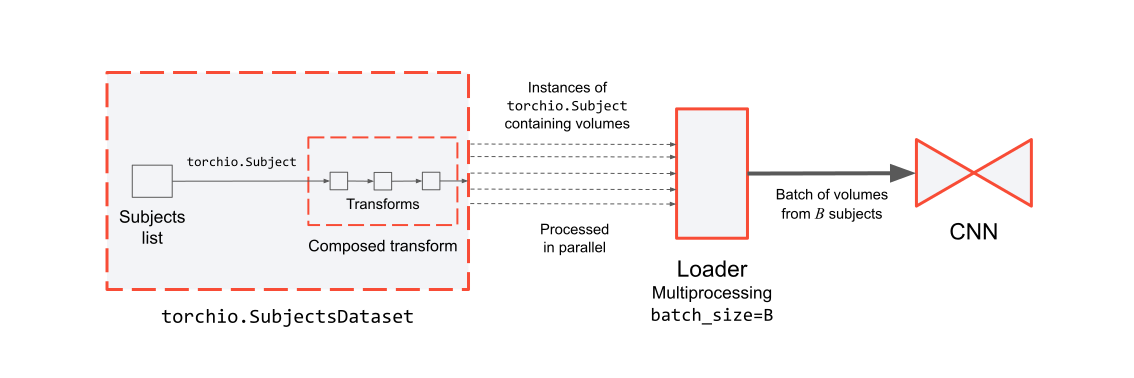
\includegraphics[width=0.9\linewidth]{Images/subjectsdataset.png}
  \caption{SubjectsDataset class and its relationships.}
  \label{fig:subjectsdataset}
\end{figure}

With these data structures, a Maxillo class, which inherit from
SubjectsDataset has been created to load the data. This class takes as input the
path of the dataset, which is split to load (train, validation, test, synthetic)
and optionally a list of Transformations that must be used as data augmentations. This class is completely independent from the rest of the code, and thus can be used in any other project which requires loading the Maxillo dataset.

\subsection{Data Augmentation}
Transformation functions that were previously defined in the same file of the
data loader have been moved to a new file. Some of them were already implemented
inside TorchIO and thus have been removed. The remaining ones have been adapted
to inherit from the abstract \texttt{class torchio.transforms.Transform}, in
order to be easily used inside TorchIO, such with the \emph{Composability}
method which allows creating a directed acyclic graph of transformations that
must be applied to the data.

\subsection{Config and command line arguments}
In the original codebase, the parameters of the program were passed both as
arguments from the command line and in the config file. This could generate some
confusion and make it harder to reproduce experiments as the config file alone
wasn't enough. For this reason, the config file is now the only source of
parameters, while the only arguments that the software accepts are the path of
the config file and a boolean value to enable/disable Tensorboard \cite{abadi2015tensorflow}.

% An example of a config file is shown below:

% \begin{lstlisting}[language=YAML,breaklines=true,caption=Example of config file., label=union]
% title: 'canal_generator_train'
% project_dir: '/homes/llumetti/results'
% seed: 47
% tensorboard_dir: '/homes/llumetti/tensorboard'

% experiment:
%   name: 'Generation'

% data_loader:
%   dataset: '/nas/softechict-nas-1/llumetti/maxillo'
%   augmentations: 'configs/augmentations.yaml'
%   background_suppression: 0
%   batch_size: 2
%   labels:
%     BACKGROUND: 0
%     INSIDE: 1
%   mean: 0.08435
%   num_workers: 8
%   patch_shape:
%   - 120
%   - 120
%   - 120
%   resize_shape:
%   - 168
%   - 280
%   - 360
%   sampler_type: grid
%   grid_overlap: 0
%   std: 0.17885
%   volumes_max: 2100
%   volumes_min: 0
%   weights:
%   - 0.000703
%   - 0.999

% model:
%   name: 'PosPadUNet3D'

% loss:
%   name: 'Jaccard'

% lr_scheduler:
%   name: 'Plateau'

% optimizer:
%   learning_rate: 0.1
%   name: 'SGD'

% trainer:
%   reload: False
%   checkpoint: null
%   do_train: False
%   do_test: False
%   do_inference: True
%   epochs: 100
% \end{lstlisting}

\subsection{Interfaces}
Something about interfaces used for Models, Losses, Optimizers, Schedulers and
Experiments...

\subsection{Deploying and Running}
The code was managed using Git and the repository is hosted on GitHub the
repository is public and can be found at
\url{https://github.com/AImageLab-zip/alveolar\_canal}. By using Git, it was
possible to easily deploy the code on the AImagelab Server by means of a simple
script that keeps the code up to date with the main branch. Other branches were
used to develop new features and to test them before merging everything in the
main branch. The Gitflow workflow was used to manage the branches. The training
was scheduled using the SLURM scheduler \cite{yoo2003slurm}, which is installed
on the server. Some scripts were written to automatize the training process,
which often required running sequentially multiple experiments with different
configuration files and to recover training from a given checkpoint when the
training was long and the scheduler kill the process for exceeding the time
limit.


% Chapter 5

\chapter{Trying to improve the State of the Art}

\lhead{Chapter 5. \emph{Trying to improve the State of the Art}} % This is for the header on each page - perhaps a shortened title
\label{chp:refwork}
%----------------------------------------------------------------------------------------

\def\:{\hskip0pt} %Definisce un modo veloce per permettere a latex di sillabare correttamente anche parole come 4-connectivity. Il corretto utilizzo è il seguente: 4\:-\:connectivity.
The architecture proposed by Cipriano et al. was quite simple yet effective. The
main novel addition was the use of positional encoding. We now want to try to
improve the results obtained by them by adding some more complex
and more recent architectures, losses, and optimizers.

\section{Boundary Loss}
Jointly with PosPadUNet3D, standard DICE loss was used. We also tried to use
CrossEntropy loss, but the results were not as good as with DICE loss so it has
been discarded. As we were dealing with highly unbalanced data, less than 1\% of
the whole volume is the canal, we looked for alternative losses which deal with
this problem.

Kervadec et al. proposed a loss function that takes the form of a distance
metric on the space of contours instead of regions. Dice or cross-entropy, are
based on regional integrals, which are convenient for training deep neural
networks. In practice, these regional integrals are summations over the
segmentation regions of differentiable functions, each directly invoking the
softmax probability outputs of the network. Therefore, standard stochastic
optimizers such as SGD are directly applicable. Unfortunately, difficulties
occur for highly unbalanced segmentations, for instance, when the size of the
target foreground region is several orders of magnitude less than the background
size, which is a common characteristic for medical images. The problem with such
losses is that they assume identical importance distribution for all the samples
and classes.

In the proposed paper, the authors proposed a new type of loss, named
\emph{Boundary loss} that aims to mitigate the issues related to regional losses
in highly unbalanced segmentation problems. Rather than using unbalanced
integrals over the regions, a boundary loss uses integrals over the boundary
between the regions. Furthermore, it provides information that is complementary
to regional losses. It is, however, challenging to represent the boundary points
corresponding to the regional softmax outputs of a CNN. This difficulty may
explain why boundary losses have been avoided in the context of deep
segmentation networks.

\subsection{Formulation}
The Boundary loss has been formulated as follows: let $I: \Omega \subset
\mathbb{R}^{2,3} \rightarrow \mathbb{R}$ denotes an image with spatial domain
$\Omega$, and $g: \Omega \rightarrow {0,1}$ a binary ground truth segmentation
of the image such that $g(p) = 1$ if the pixel $p$ belongs to the target region
$G \subset \Omega$ and $0$ otherwise. Let $s_\theta : \Omega \rightarrow [0,1]$
denotes the softmax probability output of a deep segmentation network, and
$S_\theta \subset \Omega$ denotes the corresponding segmentation region:
$\S_\theta = {p \in \Omega | s_\theta(p) >= \delta}$ for some threshold
$\delta$. Let $\Delta G$ denote a representation of the boundary of the
ground-truth region $G$ (i.e. the set of points of $G$, which have a spatial
neighbor in background $\Omega \setminus G$) and $\Delta S_\theta$ denoting the
boundary of the segmentation region defined by the network output.\\
The boundary loss can now be defined as:

\begin{equation}
  \label{eq:boundaryloss}
  \mathcal{L}_{\text{boundary}}(\theta) = \int_{\Omega} \phi_G(q)s_\theta(q)dq
\end{equation}

Where $\phi_G$ is the level set of the ground-truth region $G$, obtained by
using the signed distance transform over $G$.

\subsection{Combining with other loss functions}
As we have already said, this type of loss is complementary to the regional
losses, since it provides information about the boundary of the segmentation
region, therefore they can be combined. In our experiments, we used the
following combination:
\begin{equation}
  \label{eq:boundaryloss}
  \mathcal{L}(\theta) = (1-\alpha)\mathcal{L}_{\text{boundary}}(\theta) +
  \alpha\mathcal{L}_{\text{DICE}}(\theta)
\end{equation}
Where $\alpha$ is a hyperparameter that weights the two losses.

Kervadec et al. in the paper where they presented this type of novel loss
they've adopted a peculiar way to set this $\alpha$. As the training was kind of
unstable they set $\alpha$ to an initial value of $0$ and increased its value by
$0.01$ and each training epoch until a fixed threshold. This type of approach
have given the best results in terms of stability and performance thus we
decided to adopt it also in our experiments.

\section{PosDeepLab v3+}
DeepLab v3+ is another well-known architecture for semantic segmentation. It was
proposed by Chen et al. in 2017 with version 1. Later in the years, they
proposed small changes to the architecture, which resulted in version 2, 3, and
the latest one, version 3+. The main novelty that can be found in this
architecture is the use of Atrous Spatial Pyramid Convolutions, which are
dilated convolutions in parallel, each one with a different dilation rate and
later concatenated, the use of a fully connected Conditional Random Field, which
improves the segmentation by maximizing the label agreement between similar
pixels, and the use of depth-wise separable convolutions, which are a way to
reduce the number of parameters in the network. The model architecture is shown
in Figure \ref{fig:deeplabv3+}.
\begin{figure}[h]
  \centering
  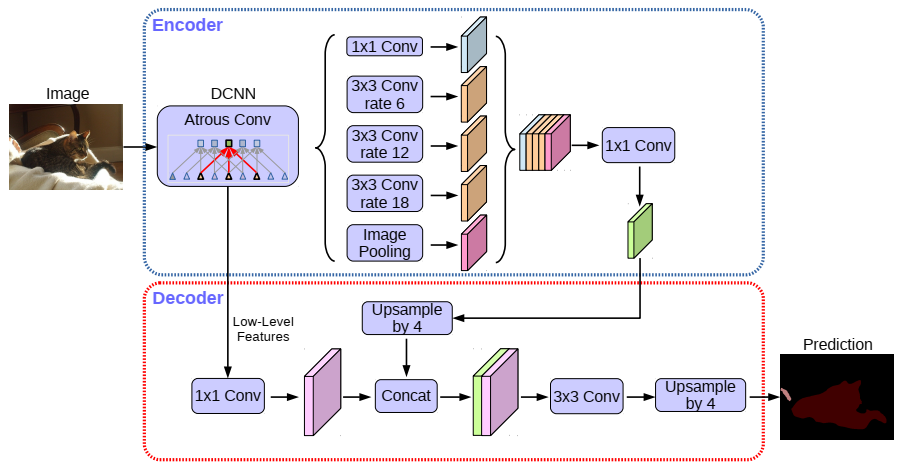
\includegraphics[width=0.8\textwidth]{Images/DeepLabv3+.png}
  \caption{DeepLab v3+ architecture}
  \label{fig:deeplabv3+}
\end{figure}

\section{PosSegNet}
SegNet is a fully convolutional network for semantic segmentation. It was
proposed by Badrinarayanan et al. in 2015 and is structured in two parts: an
encoder and a decoder, similar to the one used in the U-Net. While the encoder
is made of convolutional layers followed by max pooling. The indices of the
max pooling are stored to be used in the decoder during the upsampling.
The encoder part is made of the 13 convolutional layers of the VGG16 network,
while in the decoder always 13 layers are used, but they are made of transposed
convolutional layers. Finally, a K-class softmax classifier is used to predict
the class for each pixel.
Also in this case the same positional encoding used in PosPadUNet3D was
introduced, as it was shown to be effective in the previous architecture.
SegNet was originally proposed for the segmentation of images, but by changing
the 2D operations to 3D ones, it can be used for the segmentation of 3D volumes.
The architecture is shown in figure \ref{fig:segnet}.
\begin{figure}[h]
  \centering
  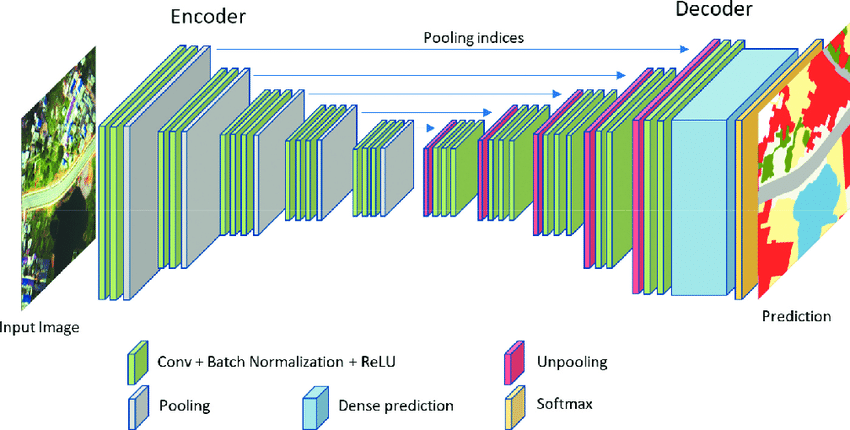
\includegraphics[width=0.5\textwidth]{Images/segnet.png}
  \caption{SegNet architecture}
  \label{fig:segnet}
\end{figure}

\section{SwinUNETR3D}
Hatamizadeh et al. recently proposed a novel architecture for 3D medical image
segmentation which make use of the Transformer architecture. The main idea is to
replace the convolutions of U-Net used in the encoding phase with Transformers.
Instead of the standard Vision Transformers, Swin Transformers have been used as
they have shown better performance on images. As Transformers are known to
suffer where there is a lack of data, also a pre-training procedure has been
proposed to overcome this problem. In the following sections, we will describe
the proposed architecture, starting from the standard Transformer as proposed in
the original paper "Attention is all you need" by Vaswani et al., and then we
will look at how these ideas have been moved from NLP to Computer Vision.

\subsection{Transformer Architecture}
The transformer architecture was first introduced by Vaswani et al. in $2017$ in
the field of Natural Language Processing. The main idea is to replace a
recurrent layer with a multi-head attention mechanism, which is a linear
operation that can be computed in parallel.
The attention mechanism is computed as follows:
\begin{equation}
  \label{eq:attention}
  \text{Attention}(Q,K,V) = \text{softmax}(\frac{QK^T}{\sqrt{d_k}})V
\end{equation}
Where $Q \in \mathbb{R}^{d_k}$ is the query, $K \in \mathbb{R}^{d_k}$ is the key
and $V \in \mathbb{R}^{d_v}$ is the value. If we would like to make it
multi-head, we add more attention layers in parallel and concatenate the
results. The final output of a multi-head attention layer is computed as
follows:
\begin{equation}
  \label{eq:multiheadattention}
  \text{MultiHeadAttention}(Q,K,V) = \text{Concat}(\text{head}_1, \dots,
  \text{head}_h)W^O
\end{equation}
where $\text{head}_i = \text{Attention}(QW_i^Q, KW_i^K, VW_i^V)$.
The projection matrices $W_i^Q \in \mathbb{R}^{d_{\text{model}} \times d_k}$,
$W_i^K \in \mathbb{R}^{d_{\text{model}} \times d_k}$, $W_i^V \in
\mathbb{R}^{d_{\text{model}} \times d_v}$, and $W^O \in \mathbb{R}^{hd_v \times
d_\text{model}}$ are learned parameters. The complete architecture, which also
adds a residual connection, a linear layer, and a normalization layer, is shown
in Figure \ref{fig:transformer}.
\begin{figure}[h]
  \centering
  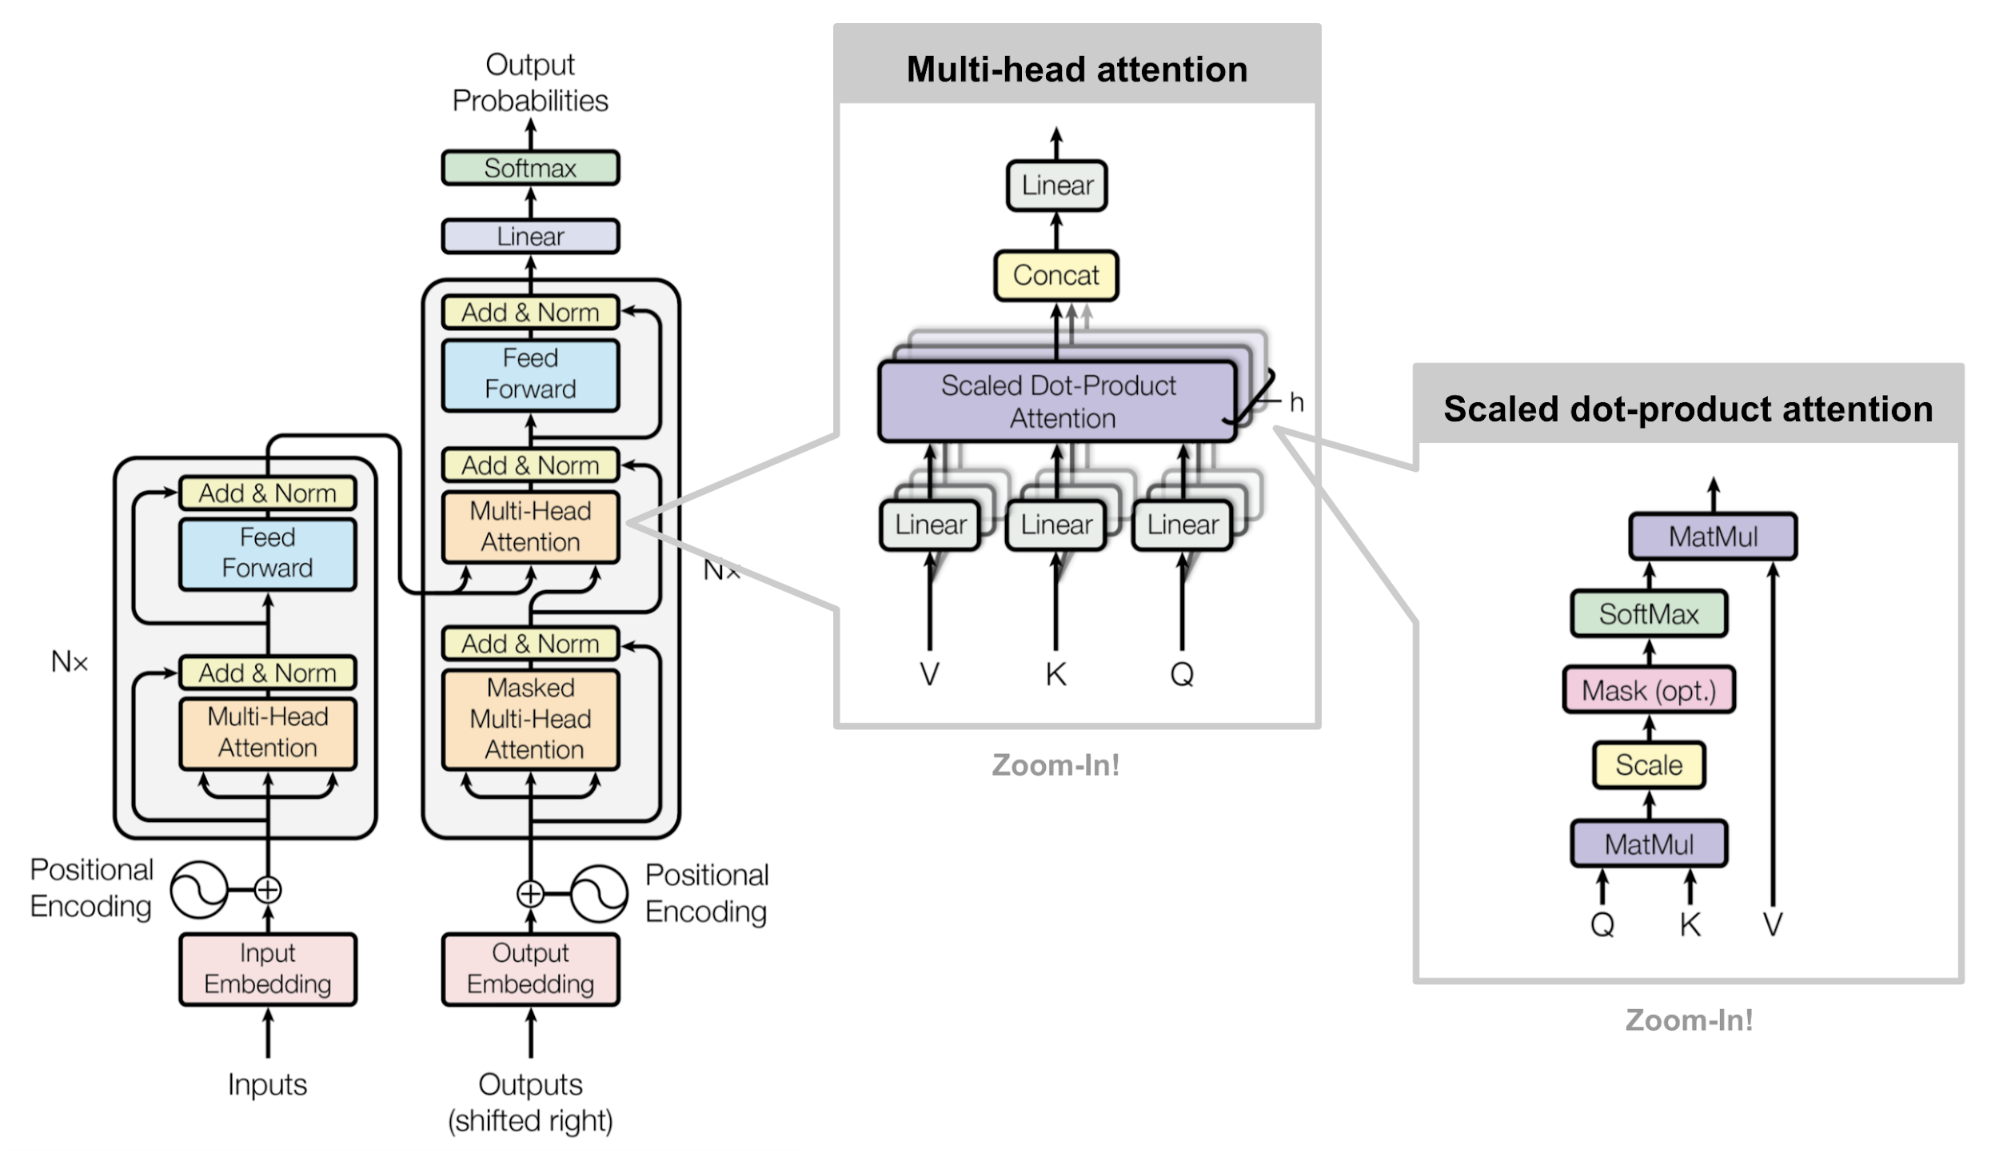
\includegraphics[width=0.8\textwidth]{transformer.png}
  \caption{Transformer architecture}
  \label{fig:transformer}
\end{figure}

\subsection{Vision Transformer}
While the Transformer architecture has become the de-facto standard for natural
language processing tasks, its applications to computer vision have remained
limited for a few years. One of the reasons is that the complexity of the
attention mechanism is $O(n^2)$, where $n$ is the number of pixels in the image.
This makes it impractical for medium and large-size images. In $2020$,
Dosovitskiy et al. proposed a novel architecture called Vision Transformer (ViT)
which is able to scale up the Transformer architecture to images. The main idea
is to reshape the original image $x \in \mathbb{R}^{H \times W \times C}$ into a
sequence of patches $x_p \in \mathbb{R}^{P \times P \times C}$, where $H$, $W$,
$C$ and $P$ are the height, width, number of channels and resolution of patches
respectively. The Transformer uses constant latent vector size $D$ through all
of its layers, so we flatten the patches and map to D dimensions with a
trainable linear projection. The outputs of such projections are patch
embeddings. An additional token \texttt{[class]} is added to the sequence, which
is used to encode the class label of the image. The whole architecture is
depicted in Figure \ref{fig:visiontransformer}.

\begin{figure}[ht!]
  \centering
  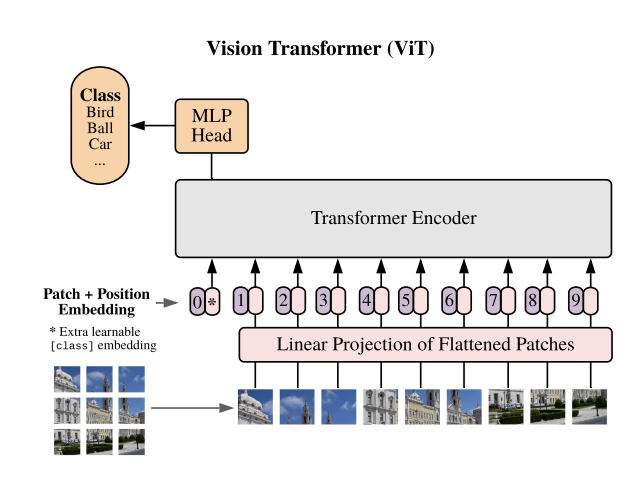
\includegraphics[width=0.5\textwidth]{Images/ViT.png}
  \caption{Vision Transformer architecture}
  \label{fig:visiontransformer}
\end{figure}


\subsection{Swin Transformer}
Swin Transformer, where the word \emph{Swin} stands for \emph{Shifted Window},
is a novel architecture proposed by Zhang et al. in $2021$ which has become
quite popular in the field of computer vision in these latter years. The problem
that the authors wanted to solve is that the Vision Transformers are not really
well suited for tasks that require dense prediction at pixel level such as
semantic segmentation, so they propose a novel that constructs hierarchical
feature maps and has linear computational complexity to image size.

The Swin Transformer still relies on patches, but instead of choosing one size
and sticking with it, it first starts with small patches for the first
Transformer layer, then merges them into bigger ones in the deeper Transformer
layers. The first size chosen for the patches is $4 \times 4$ and then it is
projected to a chosen dimensionality $C$, which in the paper has been proposed
to be $96$ for the small model and $192$ for the large model. Then, these
vectors are processed with a Transformer which makes use of a Shifted Window
based Self-Attention, introduced in this paper, instead of the classical
Self-Attention used in ViT. This type of attention has the benefit to be linear
because it is limited to a fixed number of patches $M$, so its complexity will
be $O(M \times N)$ instead of $O(N^2)$ where $N$ is the number of patches.

The output of such Transformer Layer is fed into a Merging Layer which
concatenates the vectors of groups of 2x2 neighboring patches and fed to
another Linear layer to reduce the dimensionality.
This process is repeated but for each layer, the region where the attention was
limited to is shifted in order to apply the attention to a different set of
patches, which before could not be seen among each other.

As a result, Swin Transformers are suitable for various downstream tasks wherein
the extracted multi-scale features can be leveraged for further processing.
\begin{figure}[ht!]
  \centering
  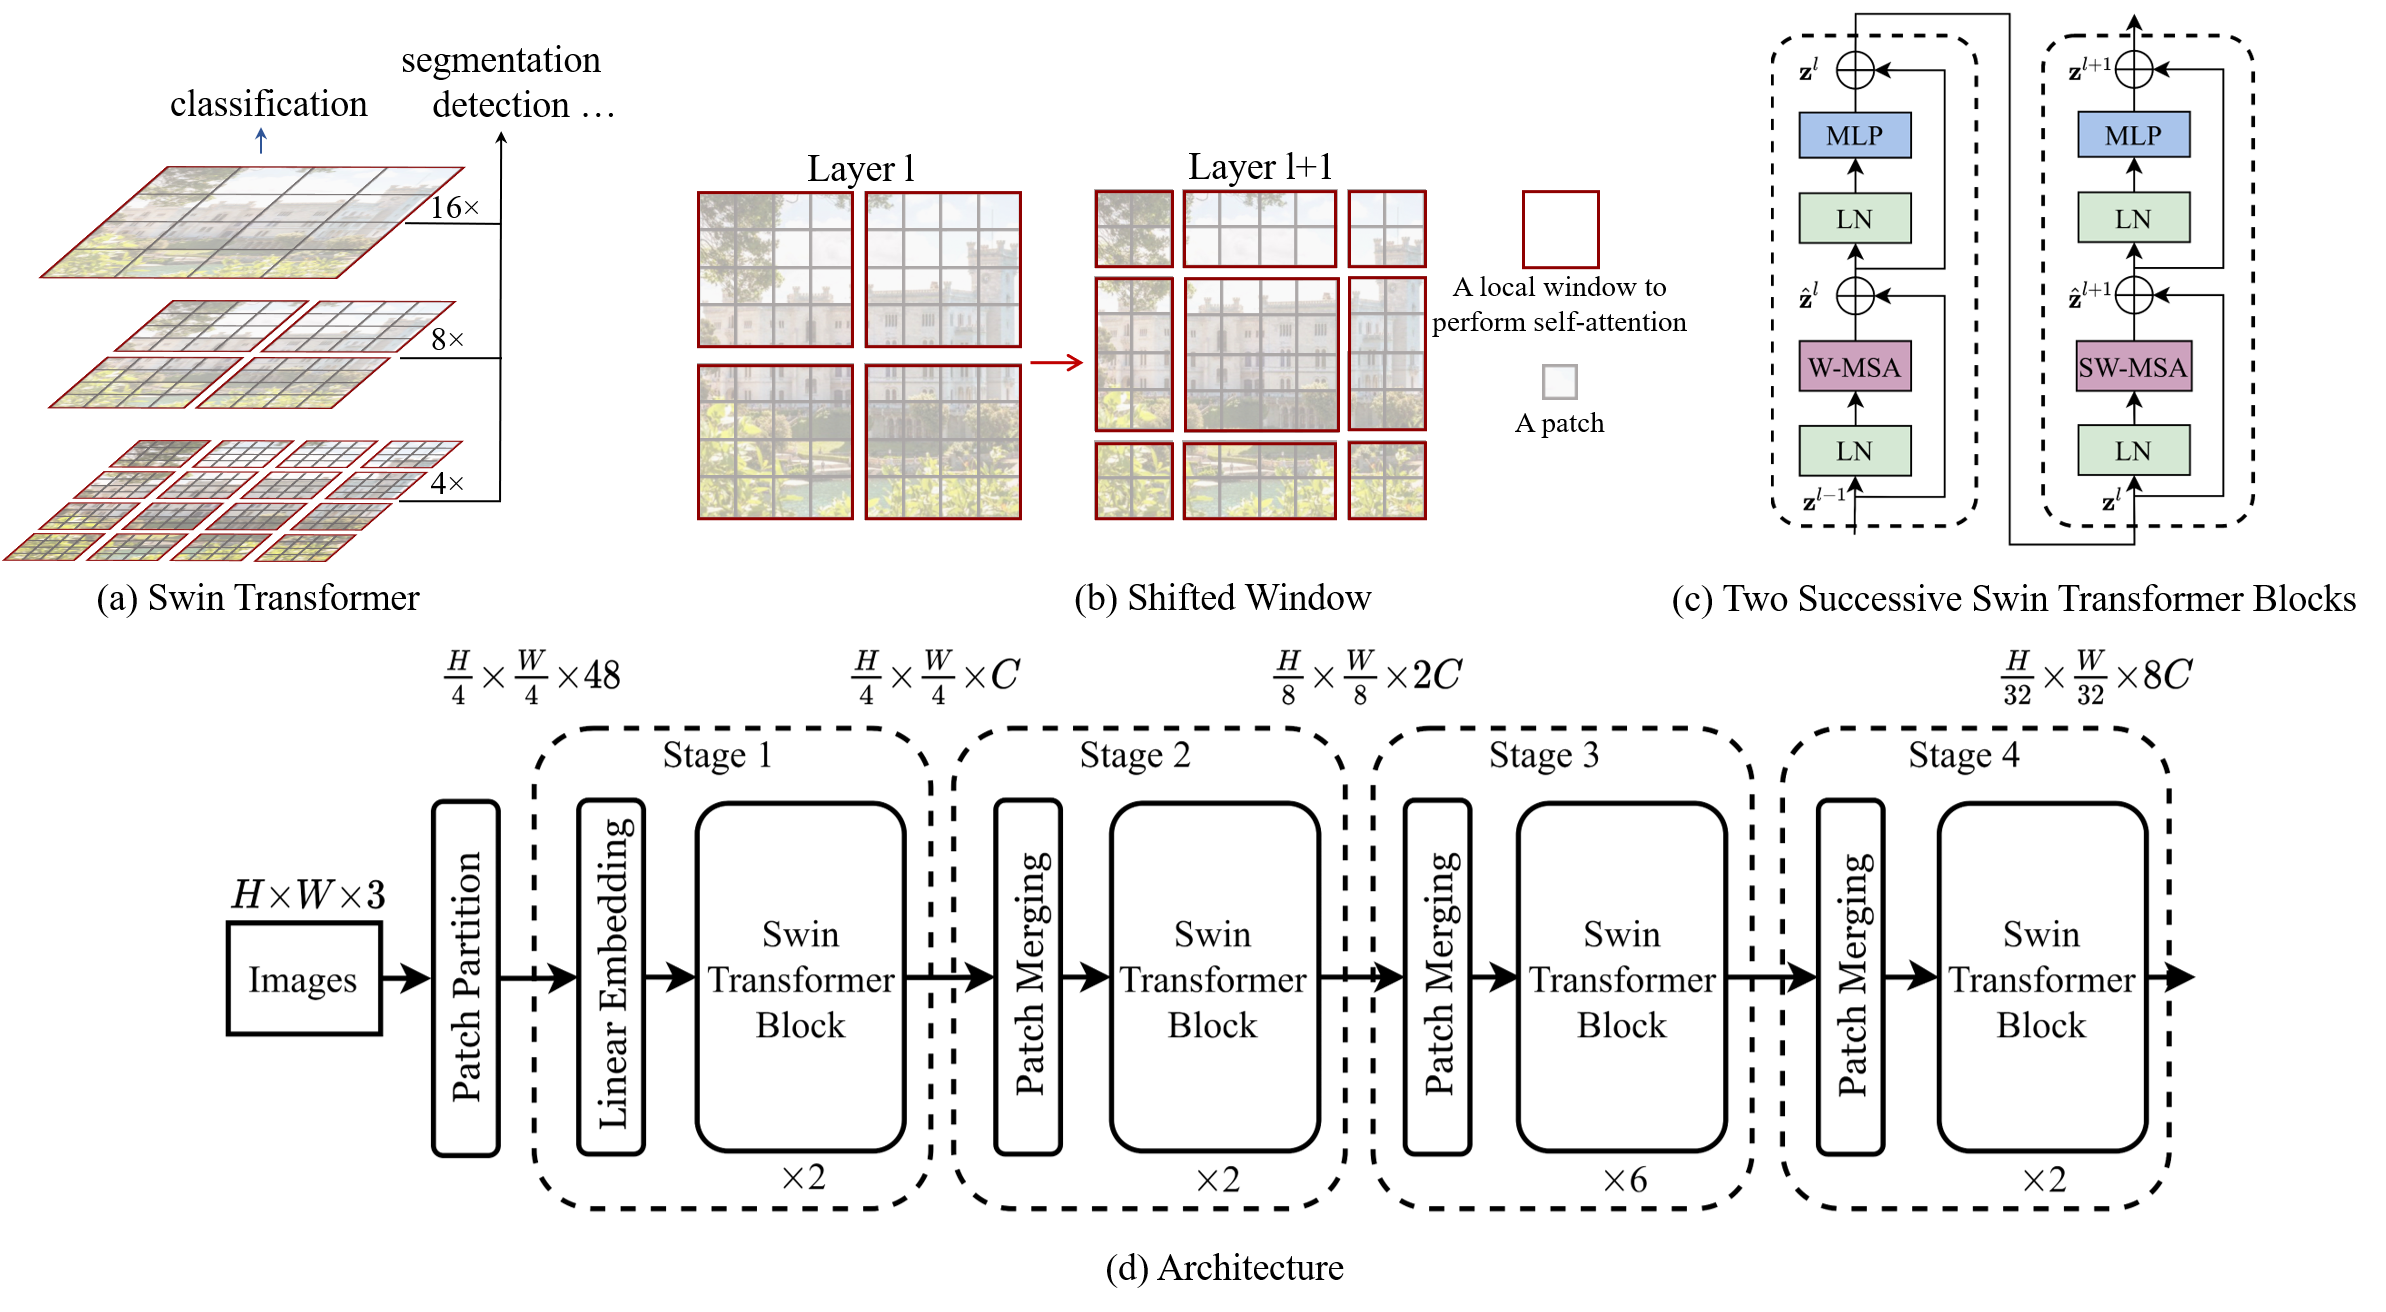
\includegraphics[width=0.8\textwidth]{Images/SwinTransformer.png}
  \caption{Swin Transformer components}
  \label{fig:swintransformer}
\end{figure}

\subsection{Final Architecture and pre-training}
The final architecture that has been proposed by Hatamizadeh et al. follows the
structure of U-Net3D, but in the encoder part, SwinTransformers are used instead
of the standard 3D Convolution. Some changes from the original paper have been
made in order to adapt the model to our type of data. From the original volume
of size $168 \times 280 \times 360$, we extract patches of size $96 \times 96
\times 96$. These patches are fed in the SwinUNetr model which is composed of a
4-stages Swin Transformer that acts as the encoder part and a sequence of
transposed convolutions as the decoder. For each stage of the encoder part, a
skip connection is added to the output of the decoder stage with the same shape,
as in the original U-Net architecture. The whole architecture is shown in Figure
\ref{fig:swinunetr}.

\begin{figure}[ht!]
  \centering
  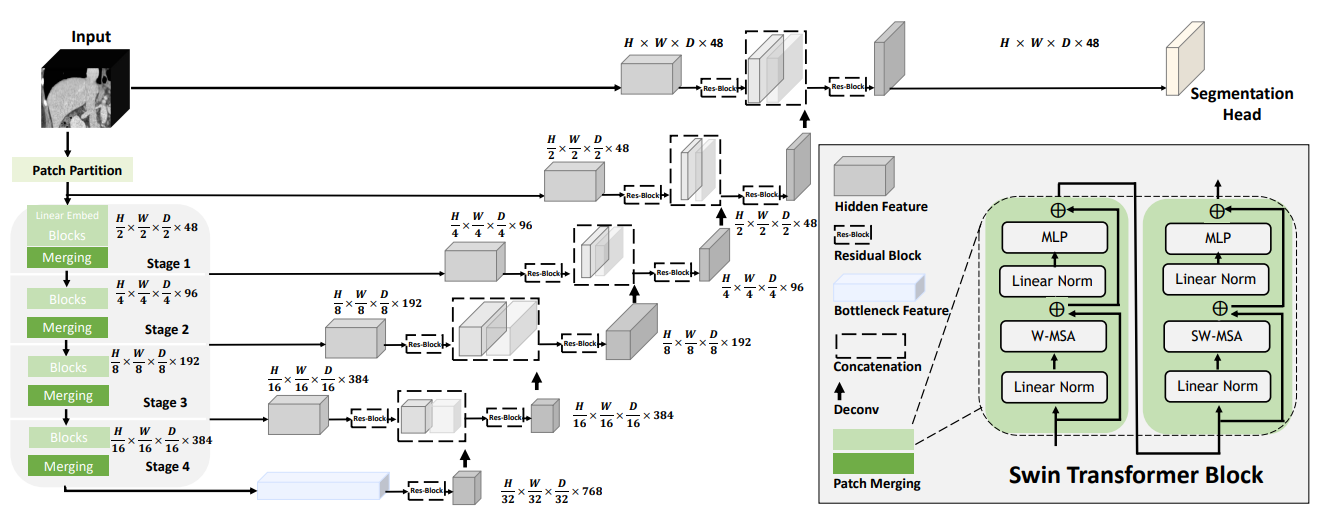
\includegraphics[width=0.8\textwidth]{Images/SwinUNETR.png}
  \caption{SwinUNETR architecture}
  \label{fig:swinunetr}
\end{figure}

As already mentioned, a pre-training phase is performed to overcome the data
hungriness characteristic of Transformers. The pretraining has been performed by
paper authors on a variety of datasets of CT scans of different types have been
used. A total of 5 public CT datasets, consisting of a total of 5,050 subjects,
are used to construct the pre-training dataset. We do not have tried to perform
the same pre-training on CBCT data instead of CT because the time required was
prohibitive.
The datasets used are:
\begin{itemize}
  \item{\textbf{Head \& Neck Squamous Cell Carcinoma (HNSCC)}: A collection
    contains imaging, radiation therapy, and clinical data from 627 head and
    neck squamous cell carcinoma (HNSCC) patients at MD Anderson Cancer Center.}
  \item{\textbf{Lung Nodule Analysis 2016 (LUNA 16)}: a collection of 888 CT
    scans of lung nodules.}
  \item{\textbf{TCIA CT Colonography Trial}: a collection of 825 CT colonography
    scans.}
  \item{\textbf{TCIA Covid 19}: a set of 2 datasets for a total of 753 CT scans
    of the chest and annotation about the Covid-19 infection.}
  \item{\textbf{TCIA LIDC-IDRI}: a collection obtained by the collaboration of
    seven academic centers and eight medical imaging companies. It contains 1018
    cases of diagnostic and lung cancer screening thoracic computed tomography
    (CT) scans with marked-up annotated lesions.}
\end{itemize}

\begin{figure}[ht!]
  \centering
  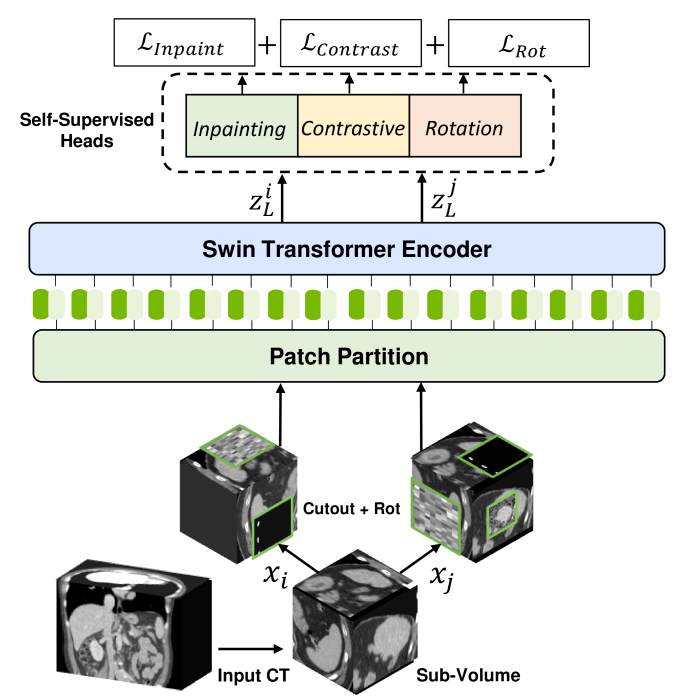
\includegraphics[width=0.4\textwidth]{Images/pretrain-unetr.png}
  \caption{Pre-training phase}
  \label{fig:pretrain-unetr}
\end{figure}
Multiple proxy tasks and formulated with a multi-objective loss function has
been used in that self-supervised phase:
\begin{itemize}
  \item{\textbf{Inpainting}: a transposed convolution layer have been attached
    to the encoder as reconstruction head, a patch is removed from the original
    volume and the model must manage to reconstruct the missing voxels, standard
    L1 loss $$\mathcal{L}_{inpaint} = ||\mathcal{X} - \hat{\mathcal{X}}||_1$$ is
    used, where $\hat{\mathcal{X}}$ is the output of the model and $\mathcal{X}$
    is the ground truth.}
  \item{\textbf{Image rotation}: The rotation prediction task predicts the angle
    categories by which the input sub-volume is rotated. For simplicity, we
    employ $R$ classes of $0$, $90$, $180$, and $270$ rotations along the
    z-axis. An MLP classification head is used for predicting the softmax
    probabilities $\hat{y}_r$ of rotation categories. Given the ground truth
    $y_r$, a cross-entropy loss is used for rotation prediction task:
    $$\mathcal{L}_{rot} = -\sum^R_{r=1}y_r\log(\hat{y}_r)$$}
  \item{\textbf{Contrastive coding}: The rotations used above where also used
    inside a contrastive loss. Given a batch of augmented sub-volumes, the
    contrastive coding allows for a better representation learning by maximizing
    the mutual information between positive pairs, while minimizing that between
    negative pairs. A linear layer is attached to the encoder to map each
    augmented sub.volume to a latent representation $v$. The cosing similarity
    is used as the distance measurement. The final loss between a pair $v_i$ and
    $v_j$ is defined as:
    $$\mathcal{L}_{contra} = -\log{\frac{\exp{(sim(v_i,v_j)/t)}}{\sum_k^{2N}1_{k
    \neq i}\exp{(sim(v_i,v_k)/t)}}}$$
    where $t$ is the measurement of normalized temperature scale. $1$ is the
    indicator function evaluating to $1 \iff k \neq i$, and $sim(\cdot, \cdot)$
    denotes the dot product between normalized embeddings.
    The contrastive learning loss function has been shown to strengthens the
    intra-class compactness as well as the inter-class separability.}
\end{itemize}

In conclusion, we minimize the final loss that is the sum of these 3 losses:
$$
\mathcal{L} = \lambda_1\mathcal{L}_{inpaint} + \lambda_2\mathcal{L}_{rot} +
\lambda_3\mathcal{L}_{contra}
$$
Where $\lambda_1$, $\lambda_2$ and $\lambda_3$ are the weights of the 3 losses
and are set to $1$ as experimentally shown to be the optimal value. In the
Figure \ref{fig:pretrain-unetr} this process is visually represented.

\section{Hann window function}
By looking at the whole segmented volume, we noticed that when using
PosPadUNet3D, the segmentation was not very accurate in the borders of each
patch. In order to solve this problem, we decided to extract overlapping patches
from the original volume instead of the non-overlapping method used in the
original paper. When two patches overlap, we would like to compute a weighted
average based on the distance from the center.
TODO: explain what happen in audio.
For this reason, we decided to apply the Hann window function to 3D volumes to
try to reduce edge effects.
\subsection{Hann window function in 1D}
The Hann window function, named after Julius von Hann, has been fist defined in
the field of signal processing, thus in 1D, as:
$$
w[n] = 0.5(1 - \cos(\frac{2\pi n}{N})), \quad n = 0, \dots, N
$$
where $x$ is the index of the window and $N$ is the total number of samples.
This function is symmetric, with a maximum value of $1$ in the middle of the
window and a minimum value of $0$ at the edges.
Another interesting property is that the sum of two Hann windows shifted by $\frac{N}{2}$
is equal to a rectangular window of width $N$ and height $1$:
$$
w[n] + w[n + \frac{N}{2}] = 0.5(1 - \cos(\frac{2\pi n}{N})) + 0.5(1 - \cos(\frac{2\pi n + N}{N} )) = 1
$$
\subsection{Hann window function in 3D}
To apply the Hann window function in 3D, we simply apply the 1D function to each
dimension of the volume:
$$
  w[x, y, z] = w[x]w[y]w[z]
$$

A cross-section of such window is shown in Figure \ref{fig:hann-window} (equivalent to a 2D window function)
% a 3x3 grid figure
\begin{figure}
  \centering
  \begin{subfigure}{0.5\textwidth}
    \centering
    %%%%%%%%%%%%
    \begin{subfigure}{.32\textwidth}
      \centering
      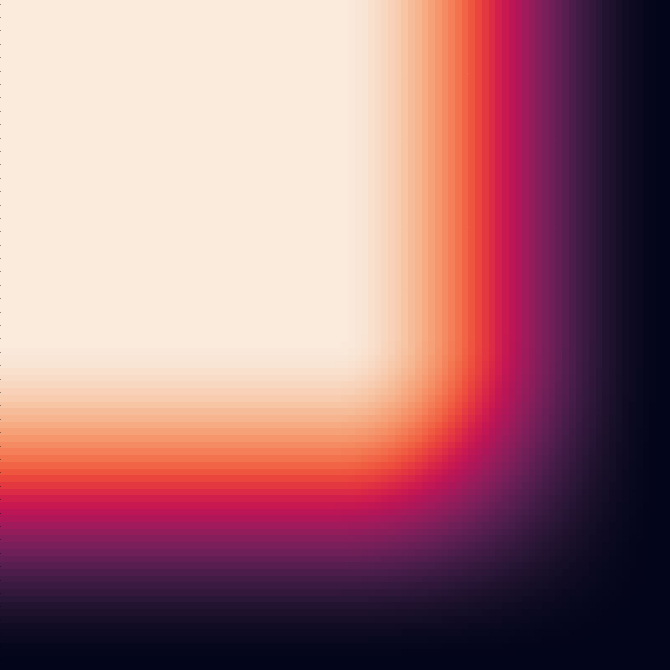
\includegraphics[width=\textwidth]{Images/hann_window_00.jpg}
    \end{subfigure}
    %%%%%%%%%%%
    \begin{subfigure}{.32\textwidth}
      \centering
      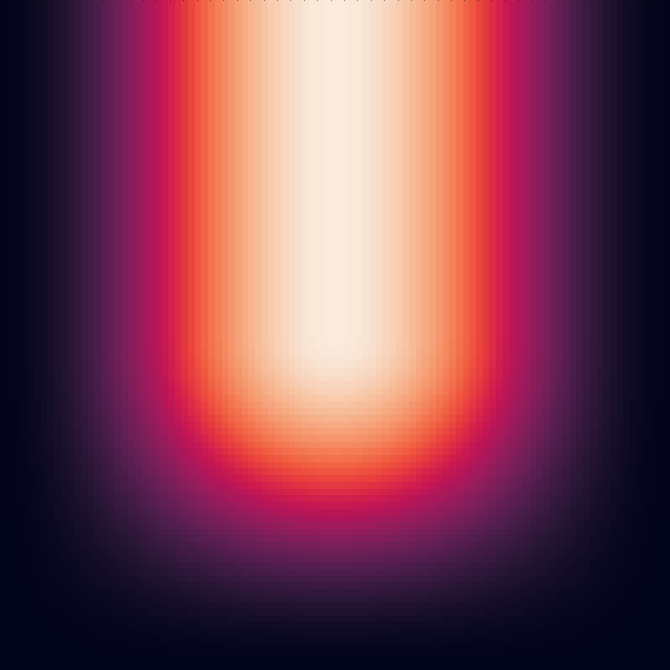
\includegraphics[width=\textwidth]{Images/hann_window_10.jpg}
    \end{subfigure}
    %%%%%%%%%%%
    \begin{subfigure}{.32\textwidth}
      \centering
      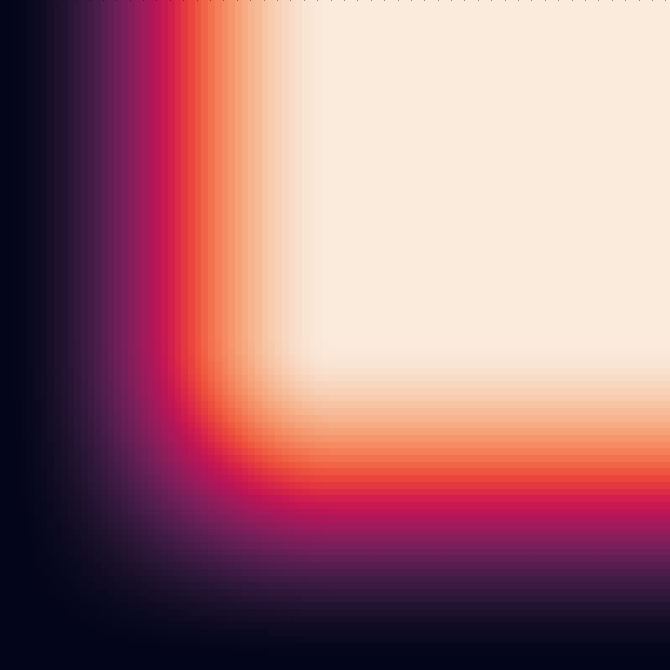
\includegraphics[width=\textwidth]{Images/hann_window_20.jpg}
    \end{subfigure}
    %%%%%%%%%%%
    \begin{subfigure}{.32\textwidth}
      \centering
      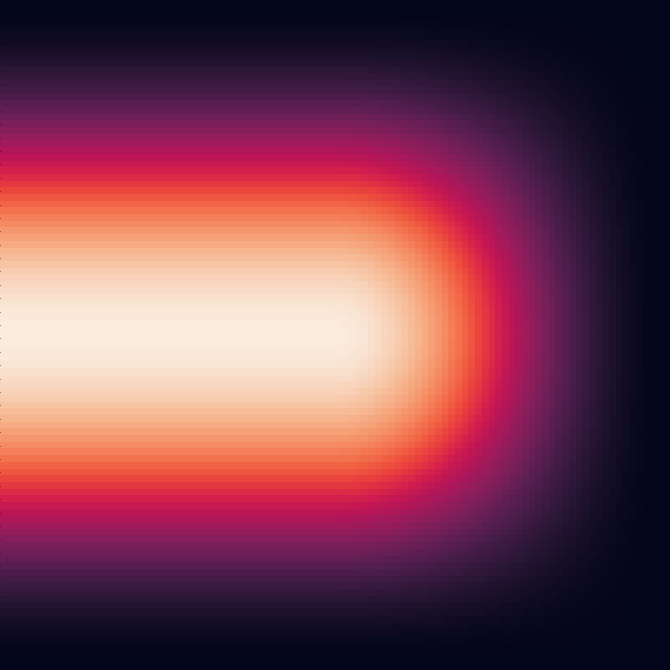
\includegraphics[width=\textwidth]{Images/hann_window_01.jpg}
    \end{subfigure}
    %%%%%%%%%%%
    \begin{subfigure}{.32\textwidth}
      \centering
      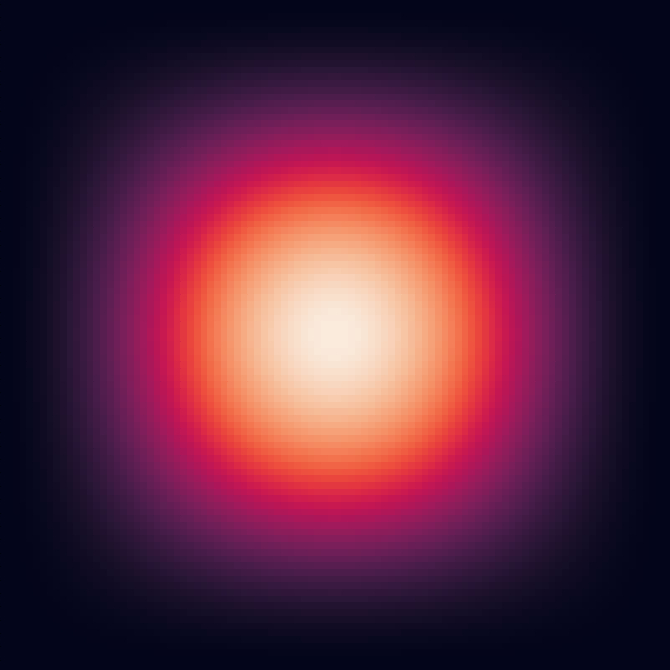
\includegraphics[width=\textwidth]{Images/hann_window_11.jpg}
    \end{subfigure}
    %%%%%%%%%%%
    \begin{subfigure}{.32\textwidth}
      \centering
      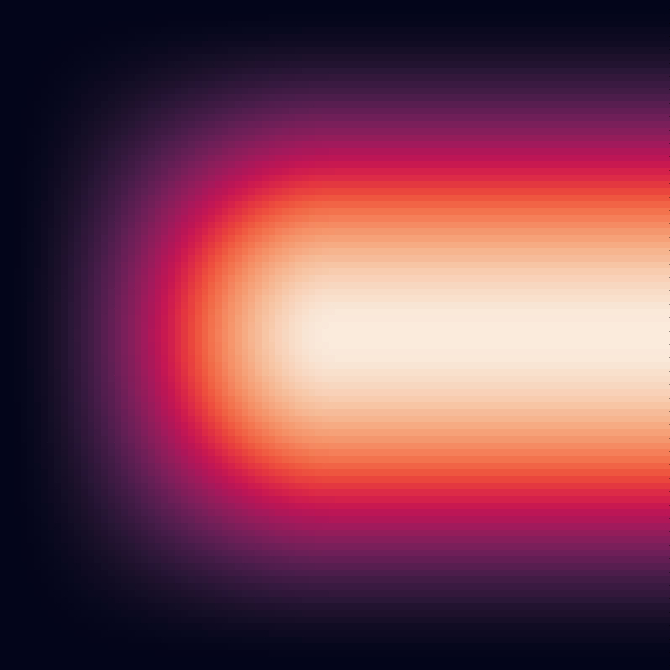
\includegraphics[width=\textwidth]{Images/hann_window_21.jpg}
    \end{subfigure}
    %%%%%%%%%%%
    \begin{subfigure}{.32\textwidth}
      \centering
      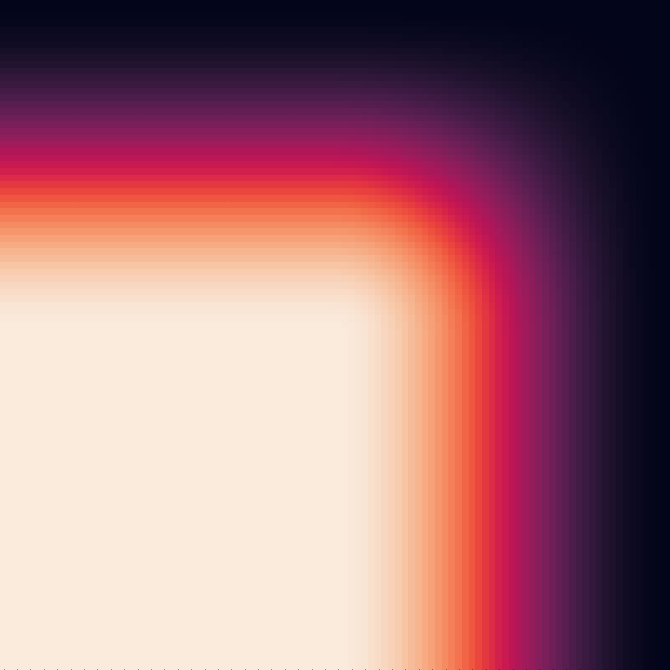
\includegraphics[width=\textwidth]{Images/hann_window_02.jpg}
    \end{subfigure}
    %%%%%%%%%%%
    \begin{subfigure}{.32\textwidth}
      \centering
      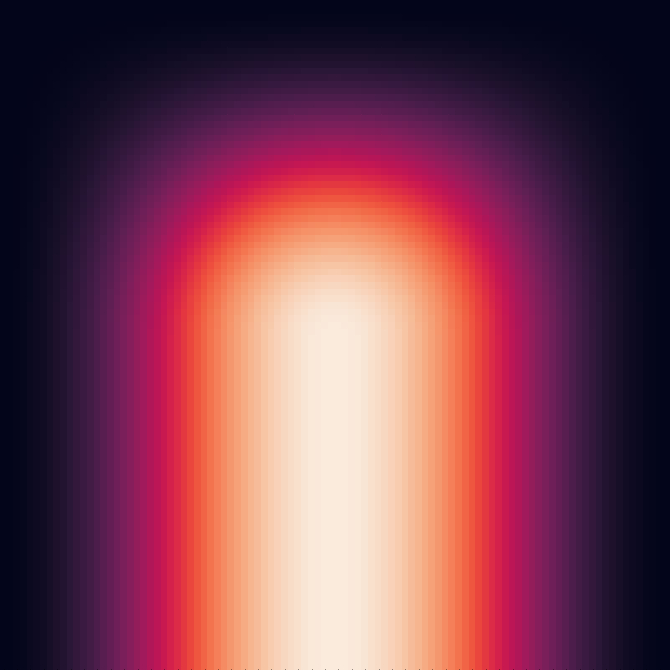
\includegraphics[width=\textwidth]{Images/hann_window_12.jpg}
    \end{subfigure}
    %%%%%%%%%%%
    \begin{subfigure}{.32\textwidth}
      \centering
      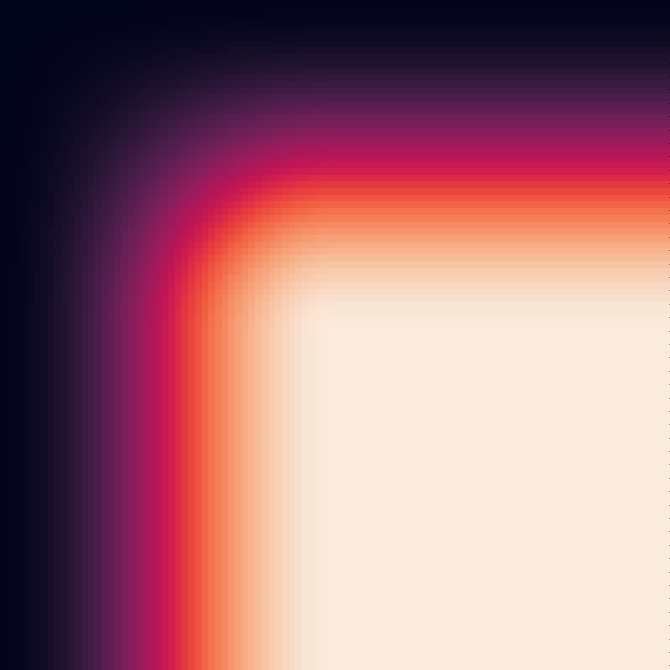
\includegraphics[width=\textwidth]{Images/hann_window_22.jpg}
    \end{subfigure}
  \end{subfigure}
  %%%%%%%%%%%
  \caption{Different Hann window functions in 2D based on the position of the extracted patch.}
  \label{fig:hann-window}
\end{figure}


\section{Performance improvements}
The last attempt made aimed to improve the performance of the model without a
excessive drop in the metrics. Being that the face of a person is symmetrical,
we decided to crop each volume in two halves, and flip the right one, then we
trained the model on both halves separately. Moreover, as the is a considerable
space between the two halves, we managed to crop a little bit more of data
leaving the canals intact. We also wanted to be able to feed a single volume
into the network without having to extract smaller patches from it. To do so, we
resize the original volume by a factor of $3$.

\section{Results}
All the models have been trained using PyTorch, on two NVIDIA P100 GPUs with 16
GB of memory, over the AImagelab server.
The model proposed by Cipriano et al. achieved the best results among the
different tries and managed to keep the title of the state-of-the-art model for
the task of segmentation of the Inferior Alveolar Canal. However, the
experiments that have been made have obtained comparable metrics thus they might
open a new path to follow to improve such results.

% A table with 

\chapter{Conclusions and future work}

\lhead{\textit{Conclusions and Future Work}} % This is for the header on each page - perhaps a shortened title

%----------------------------------------------------------------------------------------

\section{Conclusion}
\label{sec:conclusion}
The work described in this thesis has been concerned with the analysis of
extremely novel techniques for the segmentation of 3D medical images, applied to
our specific problem of segmenting the Inferior Alveolar Canal (IAC) in
cone-beam CT (CBCT) images.
After presenting the state-of-the-art in the field of image segmentation, the
work focused on improving the already existing codebase of PosPadUNet3D by
making the code more maintainable, optimizing some process of the pipeline and
by adding new features.
Finally, novel architecture proposed were implemented using PyTorch and TorchIO,
even from scratch when no code were provided in the relative paper, tested and
compared with the work carried out by Cipriano \etal.

Even if no substantial improvement regarding the metrics has been made, this
work resulted in a improvement of the code for future work and in a contribution
to the TorchIO library.

\section{Recommendation for Future Work}
All the segmentation outputs that we've got with the tested networks had in
common the lack of being a single tube for each canal that we wanted to segment.
This problem can be overcome by using shape model and asking to the network to
output the parameters for such model instead of a $H \times W \times D$
segmentation map.
Some novel loss that care about the topology of the output have been proposed,
but has not been yet widely used by the research community and hence it has not
been a priority to try during this work.
Lastly, transformers are always being more and more popular in the field of
computer vision hence the results we've got with our tests can still have some
room for improvements by getting inspired by novel approach used also in other
field such as NLP.


%----------------------------------------------------------------------------------------
%	THESIS CONTENT - APPENDICES
%----------------------------------------------------------------------------------------

\addtocontents{toc}{\vspace{2em}} % Add a gap in the Contents, for aesthetics

\appendix % Cue to tell LaTeX that the following 'chapters' are Appendices

%% Appendix A

\chapter{YACCLAB Results} % Main appendix title

\label{AppendixA} % For referencing this appendix elsewhere, use \ref{AppendixA}

\lhead{Appendix A. \emph{YACCLAB Results}} % This is for the header on each page - perhaps a shortened title

In this Appendix we report the automatic generated charts and tables from \textit{YACCLAB} project. As said before in Chapter~\ref{chp:YACCLAB}, tests were performed on each algorithm included in \textit{YACCLAB}, on all datasets, and on four different environments:

\begin{enumerate}
\item \textit{Windows} \textit{PC} with a i7-4790 \textit{CPU} @ 3.60GHz and \textit{Microsoft Visual Studio} 2013; 
\item Intel Core i7-4980HQ \textit{CPU} @ 2.80GHz running \textit{OS~X} with \textit{XCode} 7.2.1;
\item \textit{Windows} \textit{PC} with a i5-6600 \textit{CPU} @ 3.30GHz and \textit{Microsoft Visual Studio} 2013; 
\item Intel Core 2 Duo-T9600 \textit{CPU} @ 2.80GHz running \textit{OS~X} with \textit{XCode} 7.2.1. 
\end{enumerate}

Every test was repeated 10 times, and for each image the minimum execution time was considered. For a detailed discussion over results or details about the acronyms meaning see Section~\ref{sec:results}.

\clearpage

% TODO aggiornare tabelle LINUX completa
% Averages Lorenzo Windows
\begin{table}
	\centering
	\caption{Average results in ms on a i7-4790 \textit{CPU} @ 3.60GHz with \textit{Windows} and \textit{Microsoft Visual Studio} 2013 (lower is better).}
	\label{tab:appendix_ilb14_averages}
	\begin{tabular}{|l|S[table-format=2.3, table-column-width=1.5cm]|S[table-format=2.3, table-column-width=1.5cm]|S[table-format=2.3, table-column-width=1.5cm]|S[table-format=2.3, table-column-width=1.5cm]|S[table-format=2.3, table-column-width=1.5cm]|}
	\hline
	 & {SAUF} & {DiStefano} & {BBDT} & {CT} & {CCIT}\\
	\hline
	MIRflickr  & 0.611 & 0.658  & 0.261 & 0.746  & 0.295\\
    Hamlet     & 6.493 & 7.451  & 5.057 & 9.849  & 6.051\\
	Tobacco800 & 9.702 & 10.981 & 7.595 & 13.371 & 9.481\\
    Medical    & 3.469 & 3.746  & 1.983 & 4.526  & 2.457\\
    Fingerprints & 0.457 & 0.545 & 0.256 & 0.852 & 0.296\\
	3DPeS      & 0.754 & 0.844  & 0.580 & 1.015  & 0.745\\
	\hline
	\end{tabular}
\vskip 1em   
    \begin{tabular}{|l|S[table-format=2.3, table-column-width=1.5cm]|S[table-format=2.3, table-column-width=1.5cm]|S[table-format=2.3, table-column-width=1.5cm]|S[table-format=2.3, table-column-width=1.5cm]|S[table-format=2.3, table-column-width=1.5cm]|}
	\hline
	& {LSL\_STD} & {CTB} & {SBLA} & {PRED} & {NULL}\\
	\hline
	MIRflickr   & 0.464  & 0.397  & 1.451  & 0.328 & 0.187\\
    Hamlet      & 19.422 & 7.418  & 17.455 & 6.155 & 4.274\\
	Tobacco800  & 29.869 & 12.145 & 27.085 & 9.701 & 6.481\\
    Medical     & 7.564  & 3.289  & 8.506  & 2.592 & 1.710\\
    Fingerprints& 0.462 & 0.359 & 1.146 & 0.314 & 0.203\\
	3DPeS       & 2.139  & 1.046  & 2.226  & 0.802 & 0.538\\
	\hline
	\end{tabular}
\end{table}

%Average Stefano Mac
\begin{table}
	\centering
	\caption{Average results in ms on an Intel Core i7-4980HQ \textit{CPU} @ 2.80GHz running \textit{OS~X} with \textit{XCode} 7.2.1 (lower is better).}
	\label{tab:appendix_stefano_averages}
	\begin{tabular}{|l|S[table-format=2.3, table-column-width=1.5cm]|S[table-format=2.3, table-column-width=1.5cm]|S[table-format=2.3, table-column-width=1.5cm]|S[table-format=2.3, table-column-width=1.5cm]|S[table-format=2.3, table-column-width=1.5cm]|}
	\hline
	 & {SAUF} & {DiStefano} & {BBDT} & {CT} & {CCIT}\\
	\hline
    MIRflickr     & 0.420 & 0.663 & 0.296 & 0.750  & 0.349 \\
	Hamlet        & 5.710 & 6.379 & 3.969 & 8.527  & 4.861 \\
	Tobacco800    & 9.085 & 9.551 & 5.987 & 11.193 & 7.957 \\
	Medical       & 2.573 & 3.339 & 1.704 & 3.897  & 2.053 \\
	Fingerprints  & 0.340 & 0.527 & 0.297 & 0.818  & 0.339 \\
	3DPeS         & 0.519 & 0.640 & 0.416 & 0.767  & 0.495 \\
	
	\hline
	\end{tabular}
\vskip 1em   
    \begin{tabular}{|l|S[table-format=2.3, table-column-width=1.5cm]|S[table-format=2.3, table-column-width=1.5cm]|S[table-format=2.3, table-column-width=1.5cm]|S[table-format=2.3, table-column-width=1.5cm]|S[table-format=2.3, table-column-width=1.5cm]|}
	\hline
	& {LSL\_STD} & {CTB} & {SBLA} & {PRED} & {NULL}\\
	\hline
	MIRflickr     & 0.375 & 0.368 & 1.046 & 0.331 & 0.182   \\
	Hamlet        & 11.798 & 4.612 & 12.613 & 4.297 & 2.996 \\
	Tobacco800    & 23.013 & 7.554 & 19.359 & 6.693 & 4.340 \\
	Medical       & 5.662 & 2.159 & 5.897 & 1.949 & 1.282   \\
	Fingerprints  & 0.301 & 0.307 & 0.866 & 0.289 & 0.181   \\
    3DPeS         & 0.798 & 0.464 & 1.566 & 0.420 & 0.274   \\
	\hline
	\end{tabular}
\end{table}

% Averages Canci Windows
\begin{table}
	\centering
	\caption{Average results in ms on a \textit{Windows} \textit{PC} with a i5-6600 \textit{CPU} @ 3.30GHz and \textit{Microsoft Visual Studio} 2013 (lower is better).}
	\label{tab:appendix_canci_averages}
	\begin{tabular}{|l|S[table-format=2.3, table-column-width=1.5cm]|S[table-format=2.3, table-column-width=1.5cm]|S[table-format=2.3, table-column-width=1.5cm]|S[table-format=2.3, table-column-width=1.5cm]|S[table-format=2.3, table-column-width=1.5cm]|}
	\hline
	 & {SAUF} & {DiStefano} & {BBDT} & {CT} & {CCIT}\\
	\hline
	MIRflickr    & 0.776  & 0.834 & 0.409 & 0.965 & 0.508    \\
    Hamlet       & 7.717  & 8.125 & 5.309 & 9.901 & 6.376    \\
	Tobacco800   & 12.441 & 12.563 & 7.974 & 13.422 & 10.159 \\
    Medical      & 3.955  & 4.116 & 2.244 & 4.632 & 2.826    \\
    Fingerprints & 0.535  & 0.644 & 0.329 & 0.985 & 0.400    \\
	3DPeS        & 1.042  & 0.970 & 0.624 & 1.011 & 0.806    \\
	\hline
	\end{tabular}
\vskip 1em   
    \begin{tabular}{|l|S[table-format=2.3, table-column-width=1.5cm]|S[table-format=2.3, table-column-width=1.5cm]|S[table-format=2.3, table-column-width=1.5cm]|S[table-format=2.3, table-column-width=1.5cm]|S[table-format=2.3, table-column-width=1.5cm]|}
	\hline
	& {LSL\_STD} & {CTB} & {SBLA} & {PRED} & {NULL}\\
	\hline
	MIRflickr    & 1.037 & 0.521 & 1.460 & 0.492 & 0.275\\
    Hamlet       & 17.812 & 5.996 & 15.581 & 6.059 & 3.627\\
	Tobacco800   & 29.661 & 10.029 & 24.937 & 9.828 & 5.656\\
    Medical      & 7.932 & 2.820 & 7.949 & 2.680 & 1.579\\
	Fingerprints & 0.671 & 0.382 & 1.115 & 0.378 & 0.231\\
    3DPeS        & 2.217 & 0.826 & 2.002 & 0.808 & 0.455\\
	\hline
	\end{tabular}
\end{table}

% Averages Federico MAC
\begin{table}
	\centering
	\caption{Average results in ms on an Intel Core 2 Duo-T9600 @ 2.80GHz running \textit{OS~X} with \textit{XCode} 7.2.1 (lower is better).}
	\label{tab:appendix_pro_mid2009_averages}
	\begin{tabular}{|l|S[table-format=2.3, table-column-width=1.5cm]|S[table-format=2.3, table-column-width=1.5cm]|S[table-format=2.3, table-column-width=1.5cm]|S[table-format=2.3, table-column-width=1.5cm]|S[table-format=2.3, table-column-width=1.5cm]|}
	\hline
	 & {SAUF} & {DiStefano} & {BBDT} & {CT} & {CCIT}\\
	\hline
	MIRflickr    & 0.948 & 1.289 & 0.613 & 1.496 & 0.698      \\
    Hamlet       & 14.529 & 13.950 & 10.348 & 20.630 & 15.827 \\
	Tobacco800   & 25.209 & 22.553 & 18.119 & 29.343 & 28.360 \\
    Medical      & 6.041 & 6.745 & 3.931 & 8.769 & 5.700      \\
    Fingerprints & 0.678 & 1.024 & 0.567 & 1.555 & 0.611      \\
	3DPeS        & 1.078 & 1.342 & 0.984 & 1.601 & 1.120      \\
	\hline
	\end{tabular}
\vskip 1em   
    \begin{tabular}{|l|S[table-format=2.3, table-column-width=1.5cm]|S[table-format=2.3, table-column-width=1.5cm]|S[table-format=2.3, table-column-width=1.5cm]|S[table-format=2.3, table-column-width=1.5cm]|S[table-format=2.3, table-column-width=1.5cm]|}
	\hline
	& {LSL\_STD} & {CTB} & {SBLA} & {PRED} & {NULL}\\
	\hline
	MIRflickr    & 1.201 & 0.846 & 2.311 & 0.692 & 0.345\\
	Hamlet       & 35.595 & 16.016 & 24.590 & 13.846 & 6.506\\
	Tobacco800   & 63.384 & 29.564 & 37.672 & 25.560 & 10.758\\
    Medical      & 16.544 & 6.367 & 12.354 & 5.047 & 2.465\\
	Fingerprints & 0.817 & 0.649 & 1.706 & 0.583 & 0.349\\
	3DPeS        & 3.322 & 1.511 & 2.920 & 1.101 & 0.598\\
	\hline
	\end{tabular}
\end{table}

%Averages Lorenzo Windows
\begin{figure*}
\centering
\subfigure[MIRflickr] {
	\includegraphics[width=.48\textwidth]{ilb14_averages_mirflickr}
}
\subfigure[Hamlet] {
	\includegraphics[width=.48\textwidth]{ilb14_averages_hamlet}
}
\subfigure[Tobacco800] {
	\includegraphics[width=.48\textwidth]{ilb14_averages_tobacco800}
}
\subfigure[Medical] {
	\includegraphics[width=.48\textwidth]{ilb14_averages_medical}
}
\subfigure[Fingerprints] {
	\includegraphics[width=.48\textwidth]{ilb14_averages_fingerprints}
}
\subfigure[3DPeS] {
	\includegraphics[width=.48\textwidth]{ilb14_averages_3dpes}
}
\caption{Average run-time tests on a i7-4790 \textit{CPU} @ 3.60GHz with \textit{Windows} and \textit{Microsoft Visual Studio} 2013 (lower is better).}
\label{fig:appendix_ilb14_averages}
\end{figure*}

%Averages Stefano Mac
\begin{figure*}
\centering
\subfigure[MIRflickr] {
	\includegraphics[width=.48\textwidth]{stefano_averages_mirflickr}
}
\subfigure[Hamlet] {
	\includegraphics[width=.48\textwidth]{stefano_averages_hamlet}
}
\subfigure[Tobacco800] {
	\includegraphics[width=.48\textwidth]{stefano_averages_tobacco800}
}
\subfigure[Medical] {
	\includegraphics[width=.48\textwidth]{stefano_averages_medical}
}
\subfigure[Fingerprints] {
	\includegraphics[width=.48\textwidth]{stefano_averages_fingerprints}
}
\subfigure[3DPeS] {
	\includegraphics[width=.48\textwidth]{stefano_averages_3dpes}
}
\caption{Average run-time tests on an Intel Core i7-4980HQ \textit{CPU} @ 2.80GHz running \textit{OS~X} with \textit{XCode} 7.2.1 (lower is better).}
\label{fig:appendix_stefano_averages}
\end{figure*}

%Averages Canci Windows
\begin{figure*}
\centering
\subfigure[MIRflickr] {
	\includegraphics[width=.48\textwidth]{canci_averages_mirflickr}
}
\subfigure[Hamlet] {
	\includegraphics[width=.48\textwidth]{canci_averages_hamlet}
}
\subfigure[Tobacco800] {
	\includegraphics[width=.48\textwidth]{canci_averages_tobacco800}
}
\subfigure[Medical] {
	\includegraphics[width=.48\textwidth]{canci_averages_medical}
}
\subfigure[Fingerprints] {
	\includegraphics[width=.48\textwidth]{canci_averages_fingerprints}
}
\subfigure[3DPeS] {
	\includegraphics[width=.48\textwidth]{canci_averages_3dpes}
}
\caption{Average run-time tests on a i5-6600 \textit{CPU} @ 3.30GHz with \textit{Windows} and \textit{Microsoft Visual Studio} 2013 (lower is better).}
\label{fig:appendix_canci_averages}
\end{figure*}


%Averages Federico Mac
\begin{figure*}
\centering
\subfigure[MIRflickr] {
	\includegraphics[width=.48\textwidth]{pro_mid2009_averages_mirflickr}
}
\subfigure[Hamlet] {
	\includegraphics[width=.48\textwidth]{pro_mid2009_averages_hamlet}
}
\subfigure[Tobacco800] {
	\includegraphics[width=.48\textwidth]{pro_mid2009_averages_tobacco800}
}
\subfigure[Medical] {
	\includegraphics[width=.48\textwidth]{pro_mid2009_averages_medical}
}
\subfigure[Fingerprints] {
	\includegraphics[width=.48\textwidth]{pro_mid2009_averages_fingerprints}
}
\subfigure[3DPeS] {
	\includegraphics[width=.48\textwidth]{pro_mid2009_averages_3dpes}
}
\caption{Average run-time tests on an Intel Core 2 Duo-T9600 @ 2.80GHz with \textit{OS~X} and \textit{XCode} 7.2.1 (lower is better).}
\label{fig:appendix_pro_mid2009_averages}
\end{figure*}

% Density Lorenzo Windows
\begin{figure}
	\centering
	\subfigure[Density test] {
		\includegraphics[width=.59\columnwidth]{ilb14_density_cropped}
        \label{fig:appendix_ilb14_density}
	}
    \subfigure[NULL-Normalized Density test] {
		\includegraphics[width=.59\columnwidth]{ilb14_normalized_density_cropped}
        \label{fig:appendix_ilb14_normalized_density}
	}
	\subfigure[Size test] {
		\includegraphics[width=.59\columnwidth]{ilb14_size_cropped}
        \label{fig:appendix_ilb14_size}
	}
    \caption{Density, Size and NULL-Normalized Density tests on a i7-4790 \textit{CPU} @ 3.60GHz with \textit{Windows} and \textit{Microsoft Visual Studio} 2013 (lower is better).}
    \label{fig:appendix_dsn_ilb14}
\end{figure}

%Density Stefano MAC
\begin{figure}
	\centering
	\subfigure[Density test] {
		\includegraphics[width=.59\columnwidth]{stefano_density_cropped}
        \label{fig:appendix_stefano_density}
	}
    \subfigure[NULL-Normalized Density test] {
		\includegraphics[width=.59\columnwidth]{stefano_size_cropped}
        \label{fig:appendix_stefano_normalized_density}
	}
	\subfigure[Size test] {
		\includegraphics[width=.59\columnwidth]{stefano_size_cropped}
        \label{fig:appendix_stefano_size}
	}
    \caption{Density, Size and NULL-Normalized Density tests on an Intel Core i7-4980HQ \textit{CPU} @ 2.80GHz running \textit{OS~X} with \textit{XCode} 7.2.1 (lower is better).}
    \label{fig:appendix_dsn_stefano}
\end{figure}

%Density Canci Windows
\begin{figure}
	\centering
	\subfigure[Density test] {
		\includegraphics[width=.59\columnwidth]{canci_density_cropped}
        \label{fig:appendix_canci_density}
	}
    \subfigure[NULL-Normalized Density test] {
		\includegraphics[width=.59\columnwidth]{canci_normalized_density_cropped}
        \label{fig:appendix_canci_normalized_density}
	}
	\subfigure[Size test] {
		\includegraphics[width=.59\columnwidth]{canci_size_cropped}
        \label{fig:appendix_canci_size}
	}
    \caption{Density, Size and NULL-Normalized Density tests on a \textit{Windows} \textit{PC} with a i5-6600 \textit{CPU} @ 3.30GHz and \textit{Microsoft Visual Studio} 2013 (lower is better).}
    \label{fig:appendix_dsn_canci}
\end{figure}

%Density Federico Mac
\begin{figure}
	\centering
	\subfigure[Density test] {
		\includegraphics[width=.59\columnwidth]{pro_mid2009_density_cropped}
        \label{fig:appendix_pro_mid2009_density}
	}
    \subfigure[NULL-Normalized Density test] {
		\includegraphics[width=.59\columnwidth]{pro_mid2009_normalized_density_cropped}
        \label{fig:appendix_pro_mid2009_normalized_density}
	}
	\subfigure[Size test] {
		\includegraphics[width=.59\columnwidth]{pro_mid2009_size_cropped}
        \label{fig:appendix_pro_mid2009_size}
	}
    \caption{Density, Size and NULL-Normalized Density tests on an Intel Core 2 Duo-T9600 @ 2.80GHz running \textit{OS~X} with \textit{XCode} 7.2.1 (lower is better).}
    \label{fig:appendix_dsn_pro_mid2009}
\end{figure}

%% Appendix A

\chapter{Publications} % Main appendix title

\label{chp:AppendixB} % For referencing this appendix elsewhere, use \ref{AppendixA}

\lhead{Appendix B. \emph{Publications}} % This is for the header on each page - perhaps a shortened title

The research activity conducted in the context of this thesis has led to some publications in international conferences. These are summarized below and included in the following pages.

\begin{enumerate}
\item C. Grana, \textbf{F. Bolelli}, L. Baraldi, R. Vezzani. ``YACCLAB - Yet Another Connected Components Labeling Benchmark'', \textit{International Conference on Pattern Recognition - ICPR 2016}. (Submitted)
\item C. Grana, L. Baraldi, \textbf{F. Bolelli}. Optimized Connected Components Labeling with Pixel Prediction, \textit{Advanced Concepts for Intelligent Vision Systems - ACIVS 2016}. (Submitted)

\end{enumerate}

\clearpage
\pagestyle{empty}
\includepdf[pages=-,noautoscale=true,offset=85 -100,scale=0.95,pagecommand={}]{Papers/2016-icpr-yacclab.pdf}

\clearpage
\pagestyle{empty}
\includepdf[pages=-,noautoscale=true,offset=85 -100,scale=0.95,pagecommand={}]{Papers/2016-acivs.pdf}

\addtocontents{toc}{\vspace{2em}} % Add a gap in the Contents, for aesthetics

\backmatter

%----------------------------------------------------------------------------------------
%	BIBLIOGRAPHY
%----------------------------------------------------------------------------------------

\label{Bibliography}

\lhead{\emph{Bibliography}} % Change the page header to say "Bibliography"

\bibliographystyle{unsrtnat} % Use the "unsrtnat" BibTeX style for formatting the Bibliography

\bibliography{Bibliography} % The references (bibliography) information are stored in the file named "Bibliography.bib"


\end{document}
